\documentclass{article}

\usepackage[english]{babel}
\usepackage[margin=3cm]{geometry}
\usepackage{graphicx}
\usepackage{float}
\usepackage{caption}
\usepackage{hyperref}
\usepackage{amsmath}
\usepackage{wrapfig}
\usepackage[parfill]{parskip}

% fonts
\usepackage[T1]{fontenc}
\usepackage{helvet}
\renewcommand{\familydefault}{\sfdefault}

\graphicspath{{img/}}

\newcommand{\bold}[1]{\textbf{#1}}

%Define the listing package
\usepackage{listings} %code highlighter
\usepackage{upquote}
\usepackage{color} %use color
\usepackage{xcolor}
\definecolor{mygreen}{rgb}{0,0.6,0}
\definecolor{mygray}{rgb}{0.5,0.5,0.5}
\definecolor{mymauve}{rgb}{0.58,0,0.82}

% minted
\usepackage{minted}
\usemintedstyle{colorful}
\setminted{frame=single,framesep=3pt,linenos}


%Define csharp
\lstdefinelanguage{csharp}{language=[Sharp]C, frame=lrtb, rulecolor=\color{blue!80!black}}

\begin{document}

\begin{titlepage}
    \author{Tuur Vanhoutte}
    \title{Device Programming}
\end{titlepage}

\pagenumbering{gobble}
\maketitle
\newpage
\tableofcontents
\newpage

\pagenumbering{arabic}

\section{.NET}

.NET is a free, cross-platform, open source developer platform (*) for building many different types of applications.

* = languages + libraries

\begin{figure}[H]
    \centering
    \includegraphics[width=0.8\textwidth]{net-ecosystem.png}
    \caption{.NET ecosystem}
\end{figure}

\subsection{Languages}

\begin{itemize}
    \item Syntax very similar to C, C++, Java \& JavaScript
    \item Functional programming language, cross-platform, open source
    \item Approachable English-like language for Object Oriented Programming (OOP)
\end{itemize}

\subsection{Applications}

\begin{itemize}
    \item Desktop
    \item Web \& Server
    \item Mobile
    \item Gaming
    \item IoT
    \item AI
\end{itemize}

\subsubsection{Desktop}

\begin{itemize}
    \item UWP (Universal Windows Project)
    \item Xamarin.Mac
    \item WPF (Windows Presentation Foundation)
    \item WinForms (Windows Forms)
\end{itemize}

\subsubsection{Web \& Server}
\begin{itemize}
    \item ASP.NET
    \item ASP.NET Core
\end{itemize}

\subsubsection{Mobile}
\begin{itemize}
    \item UWP (Universal Windows Project)
    \item Xamarin
\end{itemize}

\subsubsection{Gaming}
\begin{itemize}
    \item Unity
    \item CryEngine
\end{itemize}

\subsubsection{IoT}
\begin{itemize}
    \item UWP
    \item .NET Core IoT
\end{itemize}

\subsubsection{AI}

\begin{itemize}
    \item Cognitive Services
    \item Azure Machine Learning
    \item Machine Learning and AI Libraries
    \item F\# for Data Science and ML
\end{itemize}

\subsection{Xamarin}
\begin{itemize}
    \item `Target all platforms with a single, shared codebase for Android, iOS, Windows'. 
    \item Developen van Mobile devices lastig: verschillende platformen, verschillende talen voor elk device.
    \item \bold{Oplossing:} Xamarin
    \item Extensie op Visual Studio.
\end{itemize}


\begin{figure}[H]
    \centering
    \includegraphics[width=0.1\textwidth]{xamarin-logo.png}
    \caption{Xamarin Logo}
\end{figure}

\subsubsection{Xamarin - UI Technology}
\begin{figure}[H]
    \centering
    \includegraphics[width=0.7\textwidth]{xamarin-forms.png}
    \caption{Native vs Xamarin.Forms}
\end{figure}

\subsubsection{Xamarin - Code Sharing strategy}

\begin{figure}[H]
    \centering
    \includegraphics[width=0.7\textwidth]{xamarin-codesharing.png}
    \caption{.NET Standard (links) vs Shared Assets Project (rechts)}
\end{figure}

Met Shared Assets Project maken we de UI voor elk platform apart. Wij gaan vooral werken met .NET Standard.


\subsection{Summary}

\begin{itemize}
    \item What devices, platforms, etc. can we target using .NET, and what programming languages can we use?
    \item What is the basic difference between .NET Standard and Shared Assets projects in Xamarin?
    \item What is the difference between Xamarin native and Xamarin.Forms? What are the advantages and disadvantages?
    \item How to set up and understand the structure of a Xamarin project for the labs in this course, and how to debug on the different platforms.
\end{itemize}

\section{C\# Syntax}

\subsection{Python vs C\# (Summary)}

\begin{itemize}
    \item Curly brackets \{ \} in plaats van indenting
    \item C\# = statically typed language: datatype is needed when declaring variables
    \begin{itemize}
        \item \underline{int} Number = 5;
        \item \underline{string} Name = "Tuur";
    \end{itemize}
    \item Python = dynamically typed language: datatype not needed
    \item C\# has more ways to create collections (Array, Dictionary, List)
\end{itemize}

\subsection{Datatypes}
\begin{figure}[H]
    \centering
    \includegraphics[width=0.7\textwidth]{csharp-datatypes.png}
    \caption{Datatypes in C\#}
\end{figure}

\subsection{Collections}
\begin{itemize}
    \item Array
    \item Dictionary<TKey, TValue>
    \item List<T>
\end{itemize}

Collection type = fixed! $\Rightarrow$ Je kan alleen objecten van het gekozen type toevoegen aan een collection

\begin{minted}{csharp}
//collections of type Person:
Person[] teacherArr = new Person[10];
List<Person> teacherList = new List<Person>();

//You can only add Person objects to these collections!
\end{minted}


\subsubsection{Arrays}
= meerdere variabelen van hetzelfde type

\begin{minted}{csharp}
//initialize int array with 10 positions:
int[] numbers = new int[10];
//save number 13 in the first position
numbers[0] = 13;
//print the value of the first number in the array:
Debug.WriteLine("The first number is:" +numbers[0]);
//intialize and fill another array with 4 numbers:
int[] startPositions = { 4, 1, 9, 3 };
\end{minted}

\subsubsection{Dictionary <TKey, TValue>}

\begin{minted}{csharp}
//declare dictionary with key type & value type
Dictionary<string, int> studentScores = new Dictionary<string, int>();
//add two elements (key value pairs)
studentScores.Add("Jean-Jacques", 13);
studentScores.Add("Jean-Louis", 4);
//get the score of Jean-Jacques
int score = studentScores["Jean-Jacques"];
\end{minted}


\subsubsection{List<T>}

\begin{minted}{csharp}
//declare list, fill one by one:
List<string> emailList = new List<string>();
emailList.Add("stijn.walcarius@howest.be");
emailList.Add("frederik.waeyaert@howest.be");
//get elements out (two ways):
string first = emailList.ElementAt(0);
string second = emailList[1];
//declare + fill list:
List<string> teacherList = new List<string> { "SWC", "FWA" };
\end{minted}

\subsection{Selections}
if / else if / else / switch

\begin{minted}{csharp}
if(findTheoryTeacher == true) {
    email1 = "frederik.waeyaert@howest.be";
    email2 = null;
}
else if(findLabTeachers == true) {
    email1 = "stijn.walcarius@howest.be";
    email2 = " frederik.waeyaert@howest.be";
} else {
    email1 = email2 = null;
}
\end{minted}

\begin{minted}{csharp}
switch (teacher){
    case "SWC":
        email = "stijn.walcarius@howest.be";
        break;
    case "FWA":
        email = "frederik.waeyaert@howest.be";
        break;
    default:
        email = "info@howest.be";
        break;
}
\end{minted}

\subsection{Loops}
for / foreach / while / do while

\begin{minted}{csharp}
for(int i = 0; i < 100; i++) {
    //do something 100 times
}
\end{minted}

\begin{minted}{csharp}
List<string> teacherList = new List<string> { "SWC", "FWA" };
foreach(string teacher in teacherList) {
    //do something
}
\end{minted}

\begin{minted}{csharp}
while(endOfClass == false){
    //might never be executed
}
\end{minted}

\begin{minted}{csharp}
do {
    //executed at least once!
} while(endOfClass == false);
\end{minted}

\subsection{Classes}
\begin{minted}{csharp}
public class Person
{
    //property
    public string Name { 
        get {...};
        set {...}; 
    }

    //constructor
    public Person(string name) {
        this.Name = name;
    }

    //method
    public void Subscribe() {
        //do something
    }
}
\end{minted}

\subsection{Instantiate objects}

\begin{minted}{csharp}
Persons p1 = new Person("Stijn");

// Based on the following constructor in the Person class:
public Person (string name) {
    this.Name = name;
}
\end{minted}

\subsection{Properties}

\subsubsection{Fields vs properties}

\begin{itemize}
    \item \bold{Fields} store the actual data
    \item \bold{Properties} are used to access those fields (getters \& setters)
    \item Auto-implemented properties have a hidden field
    \item Use properties to control field access
    \item Enhance input/output control using get \& set
    \item Calculated properties are built on other properties
    \begin{itemize}
        \item No field required
        \item Reusability
    \end{itemize}
\end{itemize}

\begin{minted}{csharp}
//private field
private int _id;

//property (zetten we altijd public)
public int Id {
    // getter
    get { return _id; }
    // setter
    set { _id = value; }
}
\end{minted}


\subsubsection{Default values for properties}

\begin{itemize}
    \item Setting default values can be useful
    \item Default values can be set\dots
    \begin{itemize}
        \item \dots with full properties
        \item \dots with auto-implemented properties
        \item \dots in the constructor
    \end{itemize}
\end{itemize}

\subsection{Constructor}

\begin{itemize}
    \item A constructor is called every time you create an instance of a class
    \item It is used to allow / force the user to provide certain values
    \item Default constructor is (only) added if a model has no constructors
    \item \bold{Constructor overloading} = multiple constructors with either \dots
    \begin{itemize}
        \item \dots a different number of parameters, or
        \item \dots a different type of parameters, or
        \item \dots the same parameters in a different order
    \end{itemize}
    \item Constructors should call each other for enhanced efficiency
    \item Constructors in inheriting classes call the constructors of the base class
\end{itemize}


\section{Streamreader}

\begin{itemize}
    \item Namespaces
    \item System.Reflection
    \item System.IO
    \item Embedded Files
\end{itemize}

\subsection{Namespaces}

Door `using' te gebruiken kunnen we de namespace weglaten:

\begin{minted}{csharp}
// Dan schrijven we:
using System.Diagnostics; // in het begin van het bestand
Debug.WriteLine("This is a debug message");
// In plaats van:
Debug.WriteLine("This is a debug message");
\end{minted}

\begin{figure}[H]
    \centering
    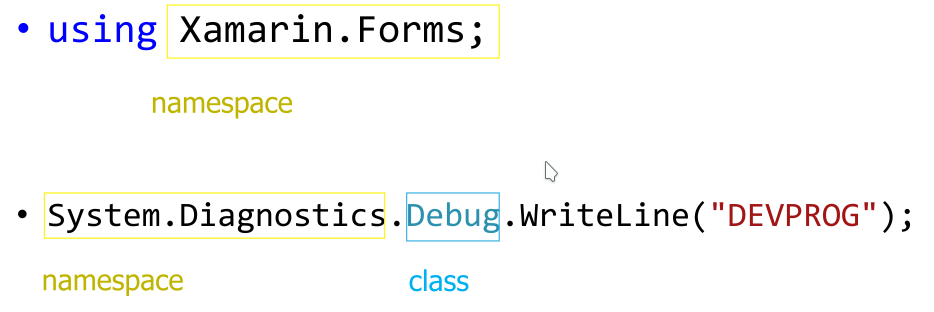
\includegraphics[width=0.5\textwidth]{namespaces.png}
    \caption{Namespaces}
\end{figure}

\subsection{System.Reflection}

\textit{"The classes in the System.Reflection namespace, together with
System.Type, enable you to obtain information about loaded
assemblies and the types defined within, such as classes, interfaces,
and value types. You can also use \bold{reflection} to create type instances
at run time and to invoke them."}

\begin{minted}{csharp}
// Using GetType to obtain type information:
int i = 42;
Type type = i.GetType();
Console.WriteLine(type);
// Output: System.Int32

// Using Reflection to get information of an Assembly:
Assembly info = typeof(int).Assembly;
Console.WriteLine(info);
// Output: System.Private.CoreLib, Version=4.0.0.0, Culture=neutral, 
    PublicKeyToken=7cec85d7bea7798e
\end{minted}

\subsection{System.IO}

= Input/Output \url{https://docs.microsoft.com/en-us/dotnet/api/system.io?view=net-5.0}

\begin{itemize}
    \item StreamReader \url{https://developer.xamarin.com/api/type/System.IO.StreamReader/}
    \begin{itemize}
        \item To read files 
    \end{itemize}
    \item StreamWriter \url{https://developer.xamarin.com/api/type/System.IO.StreamWriter/}
    \begin{itemize}
        \item To write files 
    \end{itemize}
\end{itemize}

\subsection{Embedded files}

\begin{itemize}
    \item Textfiles, images, etc.
    \item Generates a \bold{ResourceID} for the file
\end{itemize}

\begin{figure}[H]
    \centering
    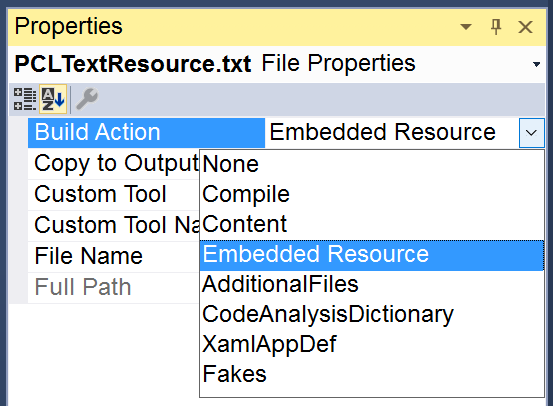
\includegraphics[width=0.3\textwidth]{embedded-files0.png}
    \caption{Embedded files inladen in een Visual Studio project: rechtermuisknop op 1 of meerdere files $\Rightarrow$ properties $\Rightarrow$ build action = Embedded resources}
\end{figure}

\subsubsection{Read an embedded file in Xamarin (using Reflection)}

\begin{figure}[H]
    \centering
    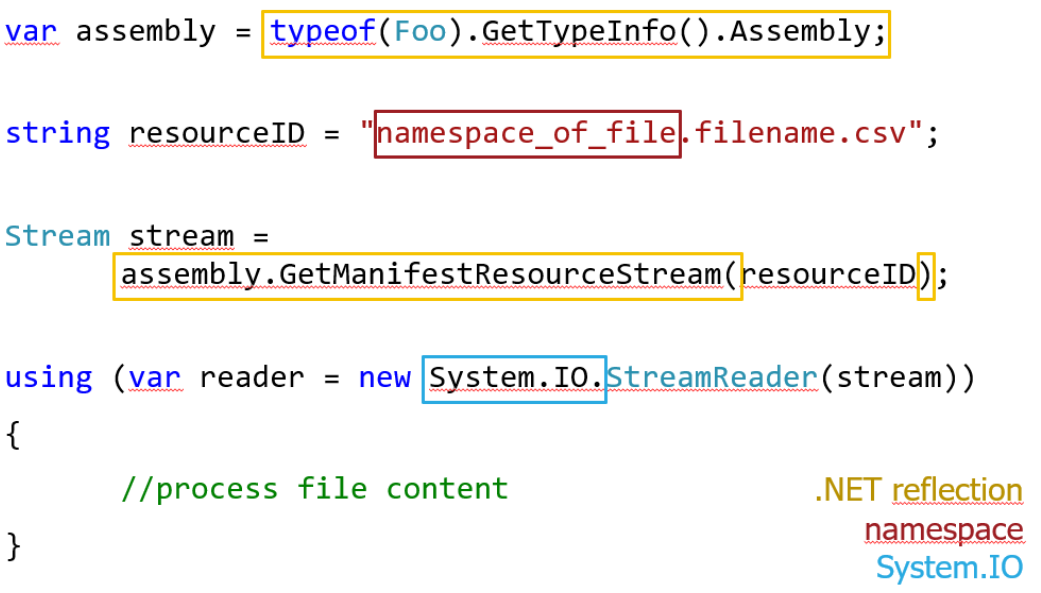
\includegraphics[width=0.6\textwidth]{embedded-files.png}
    \caption{Reading a file using StreamReader}
\end{figure}

\begin{itemize}
    \item 
\end{itemize}

\subsubsection{Processing the file's content}

\begin{figure}[H]
    \centering
    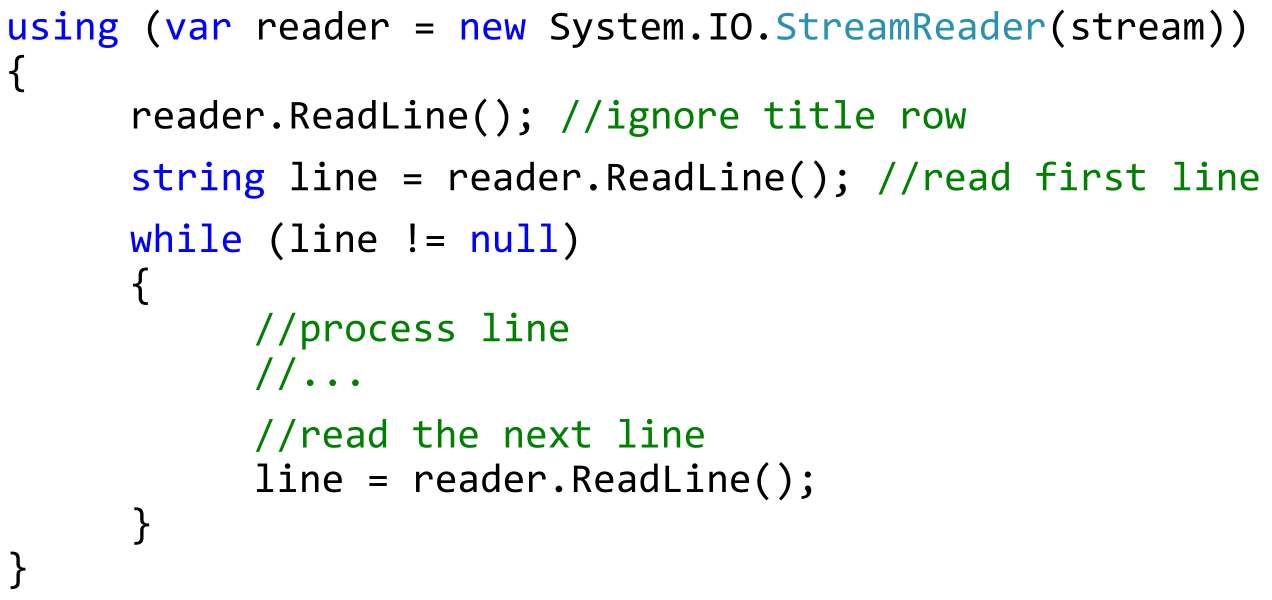
\includegraphics[width=0.6\textwidth]{embedded-files2.png}
    \caption{Processing the file's content}
\end{figure}

\subsection{Summary}

\begin{itemize}
    \item You understand the importance of \bold{namespaces}, and the techniques of using them in your own projects.
    \item You can explain the very basics of the \bold{System.IO} and \bold{System.Reflection} namespaces, and what they have to do with reading an embedded file in Xamarin.
    \item You understand the how and why of the \bold{ResourceID} that’s being generated for an embedded file.
\end{itemize}

\section{Navigation}

\subsection{Modal vs Modeless}

\begin{itemize}
    \item Modal page: requires user input to continue
    \item Modeless page: user can go back any time he wants; no input required
\end{itemize}

\begin{figure}[H]
    \centering
    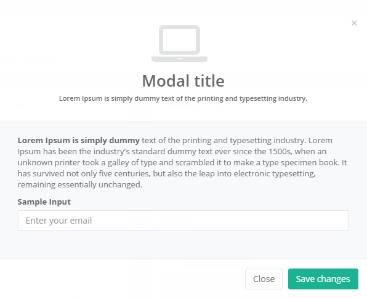
\includegraphics[width=0.5\textwidth]{modal-page.png}
    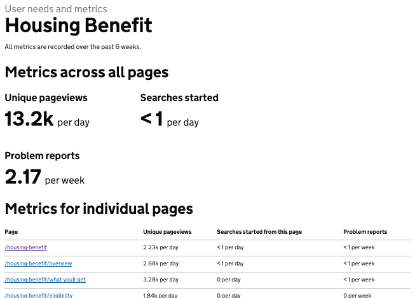
\includegraphics[width=0.4\textwidth]{modeless-page.png}
    \caption{Modal page vs Modeless page}
\end{figure}

\subsection{Navigate forward}

\begin{minted}{csharp}
Navigation.PushAsync(new FooPage());
Navigation.PushModalAsync(new FooPage());

// FooPage is hier de XAML page waar we willen naar navigeren
\end{minted}

\begin{itemize}
    \item PushAsync vs PushModalAsync
    \item Navigation object: controls the navigation stack
\end{itemize}

\subsection{Navigate back}

\subsubsection{Go back - Modeless page}

\begin{figure}[H]
    \centering
    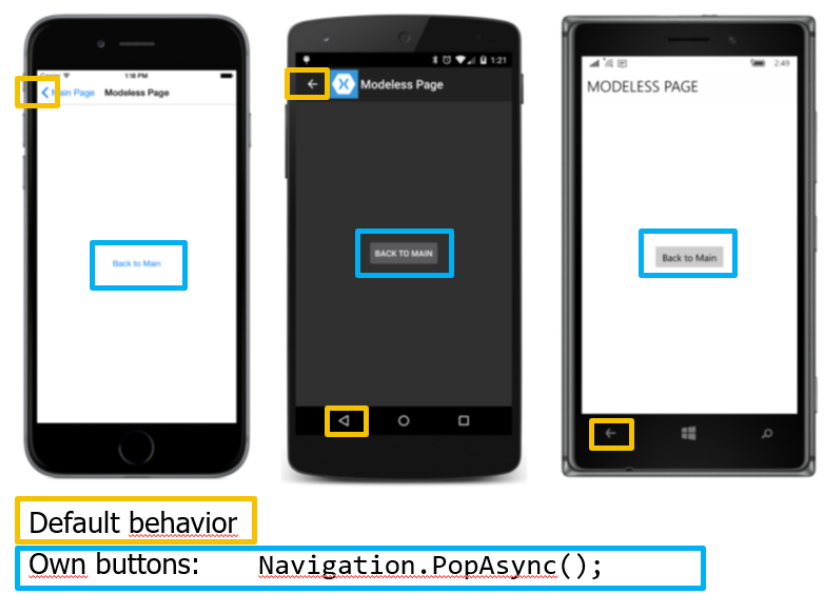
\includegraphics[width=0.5\textwidth]{navigation-back-modeless.png}
    \caption{}
\end{figure}

\subsubsection{Go back - Modal page}

\begin{figure}[H]
    \centering
    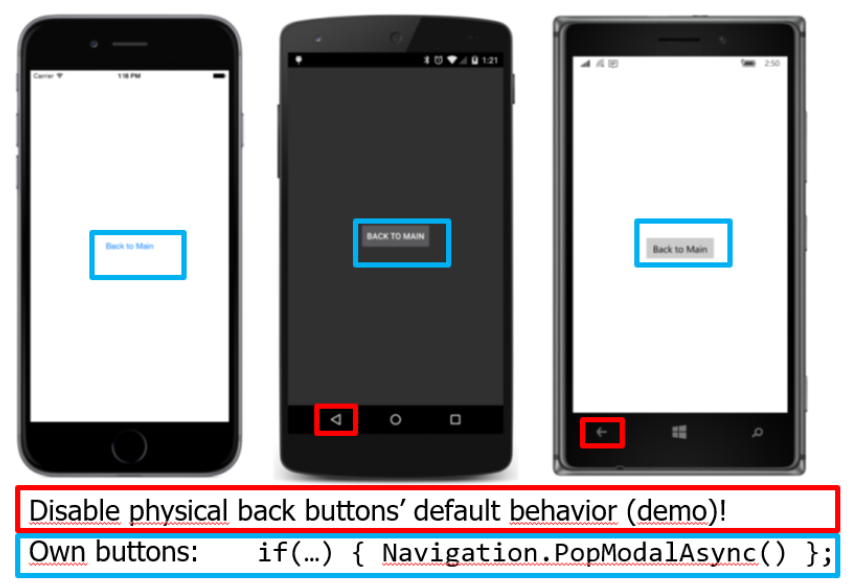
\includegraphics[width=0.5\textwidth]{navigation-back-modal.png}
    \caption{}
\end{figure}

\subsection{Navigation stack}

\begin{figure}[H]
    \centering
    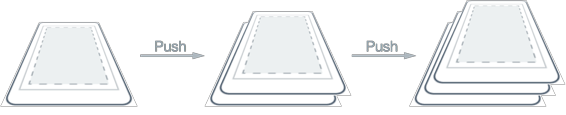
\includegraphics[width=0.4\textwidth]{navigation-stack-1.png}
    \caption{Pushing to the stack}
\end{figure}


\begin{figure}[H]
    \centering
    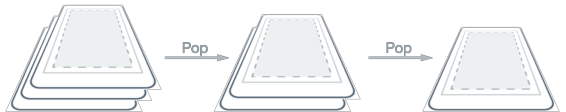
\includegraphics[width=0.4\textwidth]{navigation-stack-2.png}
    \caption{Pop-ing from the stack}
\end{figure}

\begin{figure}[H]
    \centering
    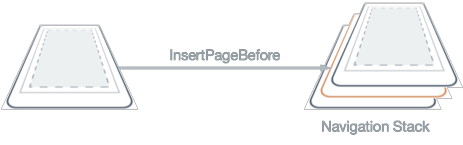
\includegraphics[width=0.4\textwidth]{navigation-stack-3.png}
    \caption{InsertPageBefore}
\end{figure}

\begin{figure}[H]
    \centering
    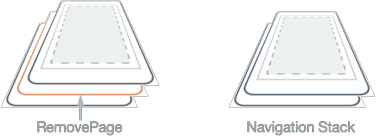
\includegraphics[width=0.4\textwidth]{navigation-stack-4.png}
    \caption{RemovePage}
\end{figure}


\begin{figure}[H]
    \centering
    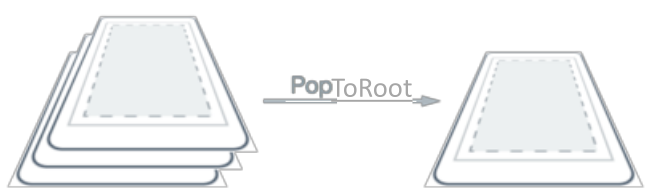
\includegraphics[width=0.4\textwidth]{navigation-stack-5.png}
    \caption{PopToRoot}
\end{figure}

\subsection{Page types}

\begin{itemize}
    \item ContentPage
    \item MasterDetailPage (zie Demo\_MasterDetail)
    \item NavigationPage (zie Demo\_Navigation)
    \item TabbedPage (zie Demo\_TabbedPage)
    \item TemplatedPage
    \item CarouselPage 
\end{itemize}

\begin{figure}[H]
    \centering
    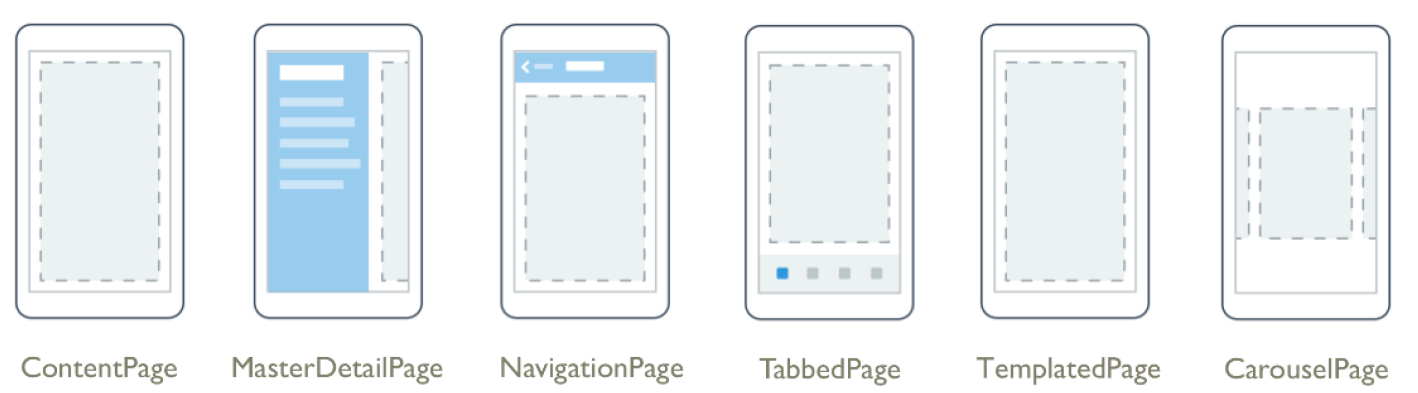
\includegraphics[width=0.8\textwidth]{pagetypes.png}
    \caption{Xamarin's page types}
\end{figure}

\subsection{Exchanging data}

How to exchange data between several pages:

\begin{enumerate}
    \item Constructor (Demo\_MasterDetail)
    \item Properties (Demo\_TabbedPage)
\end{enumerate}

\subsection{Summary}

\begin{itemize}
    \item The different \bold{page types} and how to use them.
    \item The difference between \bold{Modal} and \bold{Modeless} pages, and how to manage navigation for both.
    \item You know how to \bold{exchange data} between pages in the navigation process.
    \item You understand the \bold{navigation stack} and how you can manipulate it.
    \item You can explain the concept of a \bold{master-detail} relation with an example
\end{itemize}

\section{Object Orientation}

\subsection{Inheritance}

= klasses nemen methods en properties over van een andere klasse. 

Er ontstaat een hi\"erarchie.

\begin{minted}{csharp}
// the base class: 

public class Advisor
{
    // properties
    public string Name { get; set; }

    // methods
    public void Advise() { }
}

// the deriving class
// notice the : between the base class and deriving class

public class MinisterOfDefense : Advisor {
    // code here
}

\end{minted}

\begin{itemize}
    \item All C\# classes, of any type, are treated as if they ultimately derive from System.Object
\end{itemize}

\begin{figure}[H]
    \centering
    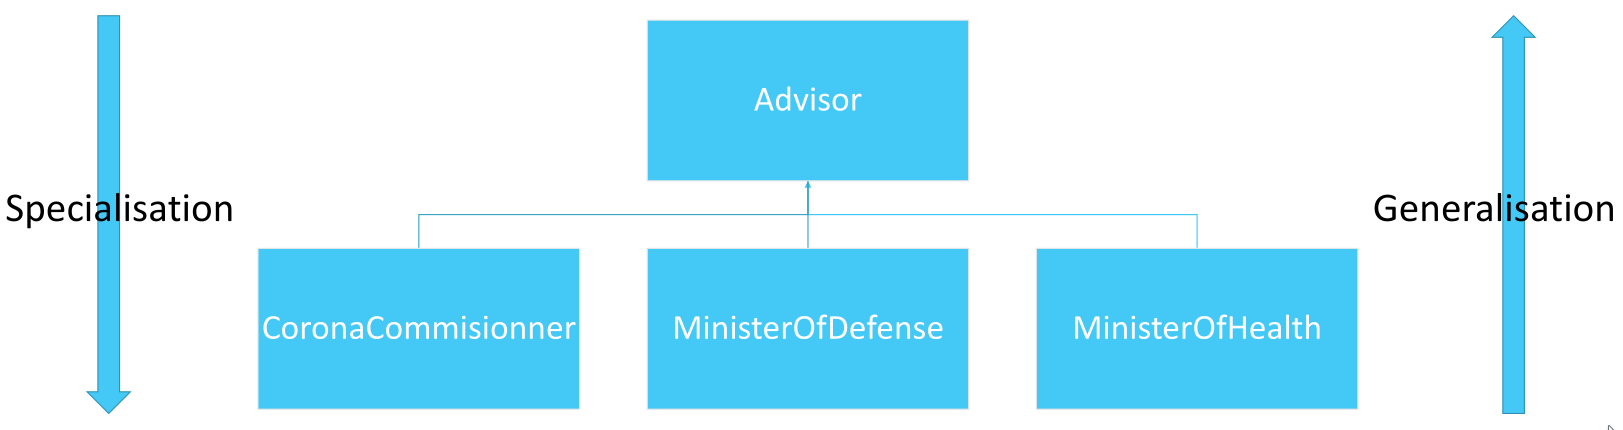
\includegraphics[width=0.75\textwidth]{inheritance.png}
    \caption{Specialisation \& Generalisation}
\end{figure}

\begin{itemize}
    \item \bold{Generalize} properties (equal for all) by putting them in the \bold{base class}
    \item \bold{Specify} properties (specific for one) by putting them in the \bold{deriving class}
\end{itemize}

\subsubsection{Constructor}

\begin{itemize}
    \item Constructors are \bold{not} inherited!
    \item Constructor without parameter in base class?
    \begin{itemize}
        \item $\Rightarrow$ Automatically called by deriving class
    \end{itemize}
    \item No constructor without parameters in base class?
    \begin{itemize}
        \item $\Rightarrow$ Explicitly call it in deriving classes
    \end{itemize}
\end{itemize}

\begin{figure}[H]
    \centering
    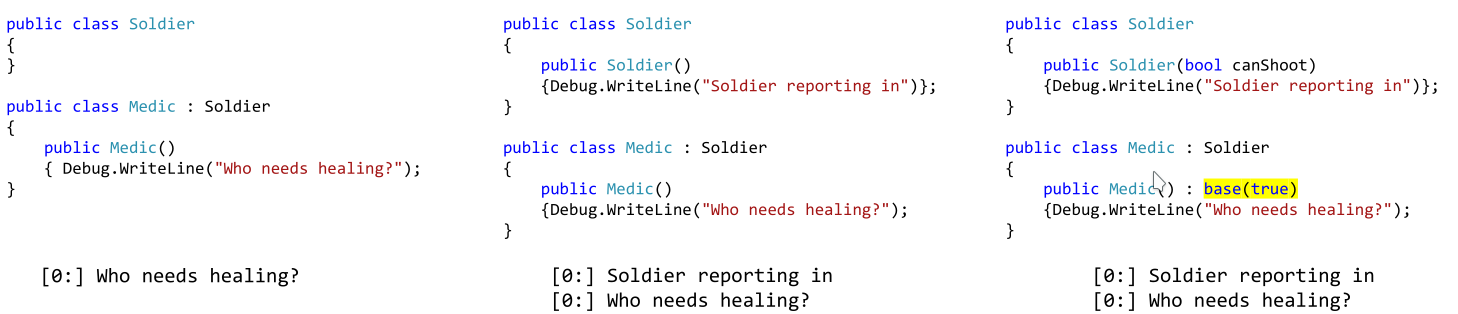
\includegraphics[width=0.95\textwidth]{inheritance-constructor.png}
    \caption{Inheritance: constructor example}
\end{figure}

\subsubsection{Access modifiers}

public is the default access modifier.

\begin{figure}[H]
    \centering
    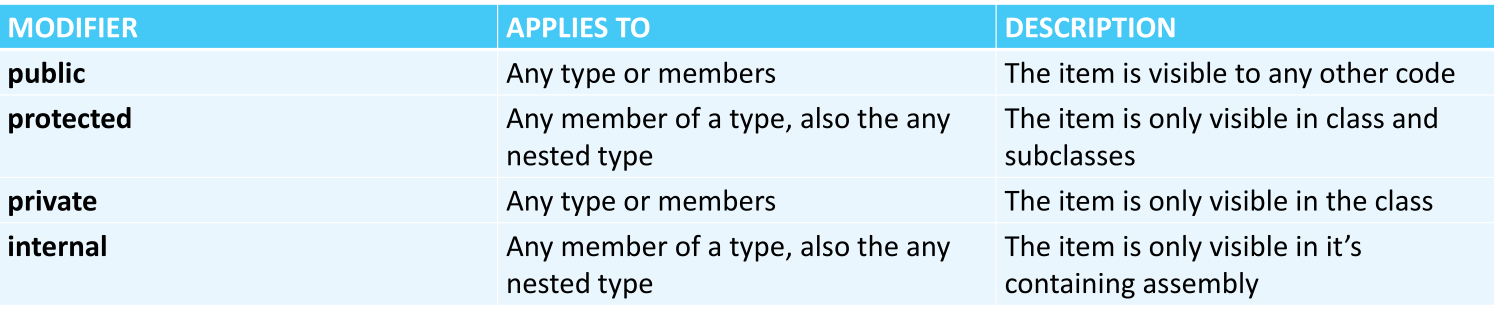
\includegraphics[width=0.9\textwidth]{inheritance-access-modifiers.png}
    \caption{Inheritance: access modifiers}
\end{figure}

\subsubsection{Properties/methods: VIRTUAL and OVERRIDE}

When you want to override a method from the base class, 
use the \bold{virtual} keyword in the base method,
and the \bold{override} keyword in the derived method.

Virtual properties/methods:
\begin{itemize}
    \item Default implementation in base class
    \item `virtual' keyword, to \bold{replace} the way an object behaves
    \item \bold{CAN} be overriden in subclasses, only if necessary.
\end{itemize}

\begin{figure}[H]
    \centering
    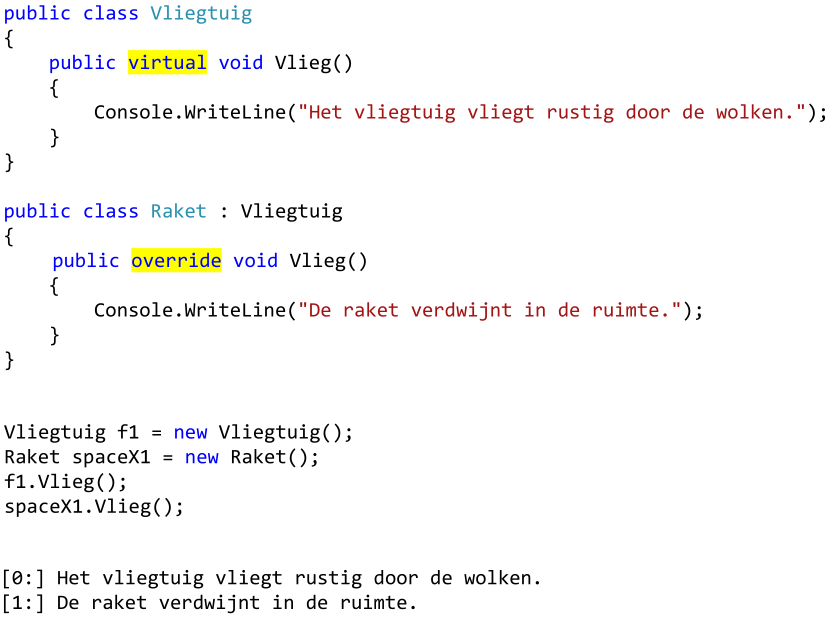
\includegraphics[width=0.9\textwidth]{inheritance-override.png}
    \caption{virtual and override}
\end{figure}


\subsubsection{Properties/methods: ABSTRACT and OVERRIDE}

Abstract properties/methods:

\begin{itemize}
    \item No default implementation possible in base class
    \item `abstract' keyword, to \bold{extend} the way an object behaves
    \item \bold{MUST} be present in each deriving class
\end{itemize}

\begin{figure}[H]
    \centering
    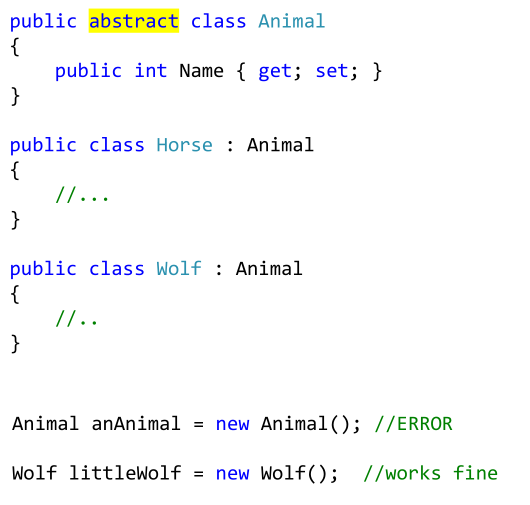
\includegraphics[width=0.4\textwidth]{inheritance-abstract.png}
    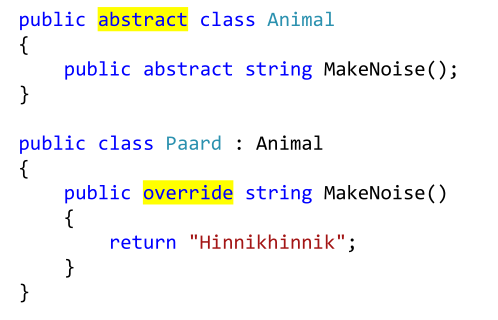
\includegraphics[width=0.4\textwidth]{inheritance-abstract2.png}
    \caption{abstract and override}
\end{figure}


\subsection{Polymorphisme}

= Objects of a derived class can be treated like objects of the base class at runtime

\bold{Example:} say we have a class Animal, and two classes Cat and Dog that inherit the Animal class.
Then, this is possible: 

\begin{minted}{csharp}
List<Animal> animals = new List<Animal>();
Animal dog = new Dog();
Animal cat = new Cat();

animals.Add(dog);
animals.Add(cat);
\end{minted}

\begin{figure}[H]
    \centering
    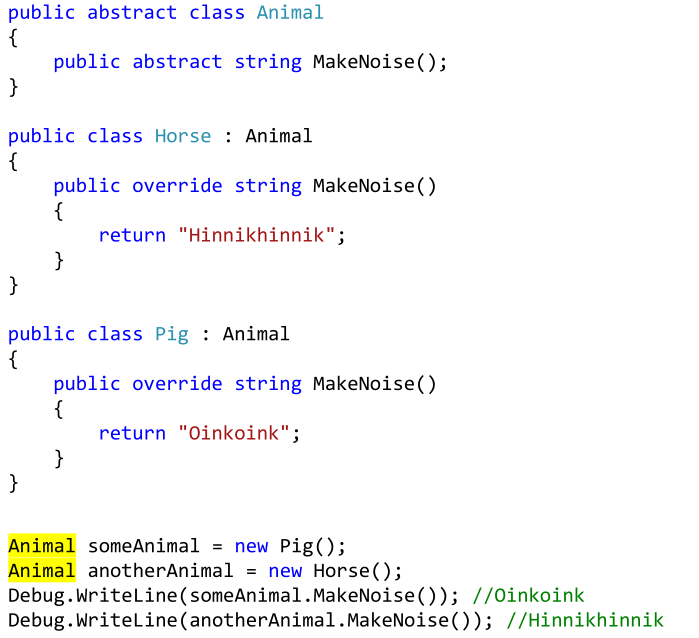
\includegraphics[width=0.8\textwidth]{polymorphism.png}
    \caption{Polymorphism example}
\end{figure}

\subsubsection{Disadvantage}

\textcolor{red}{!!!} \bold{Multiple inheritance} is \bold{NOT} allowed through classes in C\# \textcolor{red}{!!!}

\subsection{Interfaces}

\begin{itemize}
    \item Interfaces can be seen as contracts for classes
    \item Implementing = applying the contract
    \item An interface \bold{forces} all implementing classes to implement \bold{all} properties and/or methods
    \item An interface has no default implementation on its own (=you can't create an instance from an interface)
\end{itemize}

\begin{minted}{csharp}
// You can't create an instance from an interface:
interface IAdvisor{
    void Advise();
}

// This will create an error:
IAdvisor advisor = new IAdvisor();
\end{minted}

\subsubsection{Summary}

\begin{itemize}
    \item Contract + NO implementations = interface
    \item Contract + SOME implementations = abstract (base) class
    \item Implementation for all properties \& methods = normal (base) class
\end{itemize}

\subsubsection{Example}

\begin{itemize}
    \item The IAdvisor interface has an Advise() method (notice that method has no default implementation)
    \item Every class that implements this interface also must have its own Advice() method
    \item A class can implement multiple interfaces (see the MicrosoftCEO class)
    \item In the PrimeMinister class:
    \begin{itemize}
        \item A list is created with the same type as the interface
        \item Every element in that list is of a class that implements the interface
        \item Can therefore also be used in a foreach() loop
    \end{itemize}
\end{itemize}

\begin{figure}[H]
    \centering
    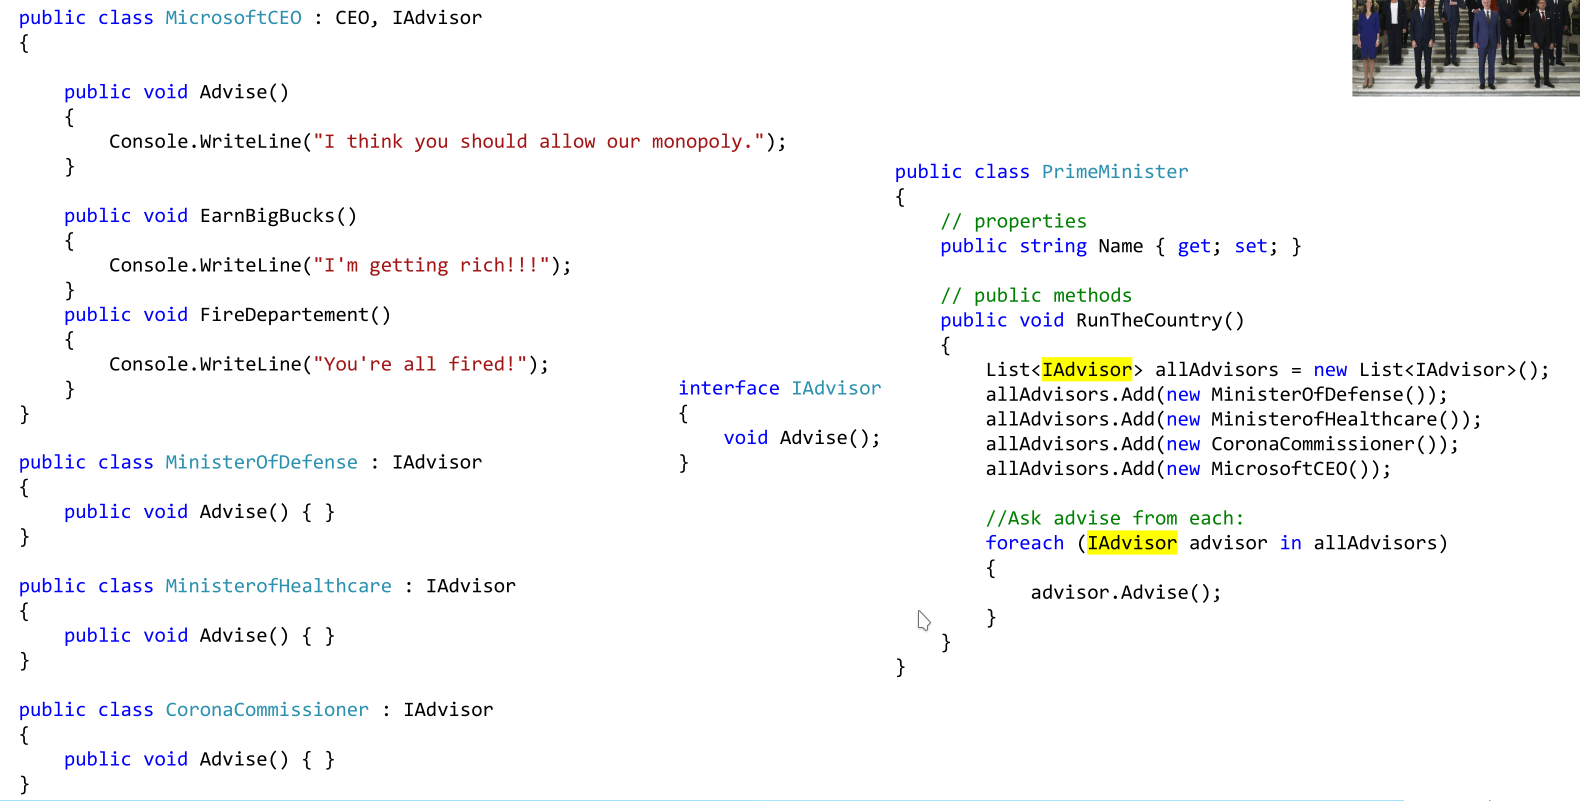
\includegraphics[width=\textwidth]{interfaces.png}
    \caption{Interfaces example}
\end{figure}

\subsection{Composition vs Aggregation}

= Creating an instance of an object from a class in another class.

\subsubsection{Example}

\begin{figure}[H]
    \centering
    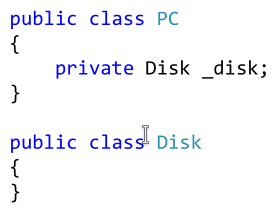
\includegraphics[width=0.3\textwidth]{composition1.png}
    \caption{How can we make an instance of `\_disk'?}
\end{figure}

\begin{figure}[H]
    \centering
    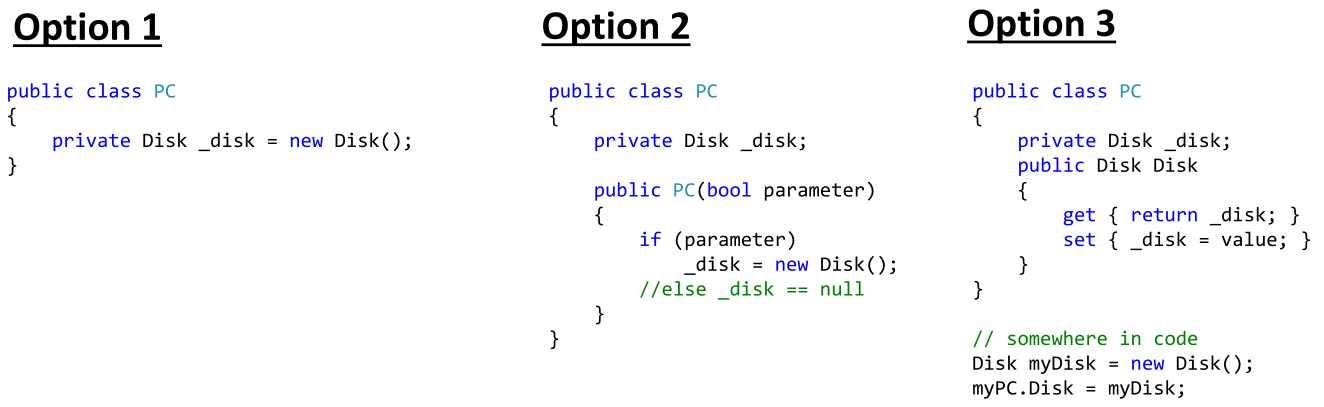
\includegraphics[width=0.85\textwidth]{composition2.png}
    \caption{Solution: 3 options}
\end{figure}

\bold{Option 1:} creating it at the start of the class (=composition)

\bold{Option 2:} using the constructor (=composition)

\bold{Option 3:} Outside of the class, by creating a new object an assigning that object to the `\_disk' property in the class.

The 3rd option is called \bold{Aggregation}. Unlike the other options, the `myDisk' object keeps existing even if the PC class stops existing.

\subsubsection{Interfaces in Xamarin(.Forms)}

Interfaces in Xamarin(.Forms) is extremely useful: 

Say you need to get data from a specific sensor on your Android/iOS/UWP device. 
We can create an interface in our project, and implement that interface in each device's code.
Once we need to get that data, we can automatically call the correct method for the correct device.

\subsection{Summary}

\begin{itemize}
    \item You are convinced by the advantages of \bold{inheritance} and \bold{polymorphism}, and can explain using an example.
    \item You understand the usage and consequences of the \bold{virtual} and \bold{abstract} keywords for properties and methods.
    \item You know when to use \bold{abstract classes} and/or \bold{interfaces}, and can explain the difference between those two.
    \item You understand the specific importance of interfaces in \bold{Xamarin}(.Forms)
\end{itemize}

\section{Asynchronous programming: async and await keywords}

\subsection{Why?}

To make the app continue to respond to use interaction while\dots:
\begin{itemize}
    \item \dots Reading from or writing to a database or file
    \item \dots Accessing a web service
    \item \dots Performing data processing
\end{itemize}

\subsection{Example: newspaper app}

\begin{itemize}
    \item Load the trending newspaper items
    \item Load user preferences
    \item Load newspaper items based on preferences $\Rightarrow$ needs to wait until user preferences are set
\end{itemize}

\begin{figure}[H]
    \centering
    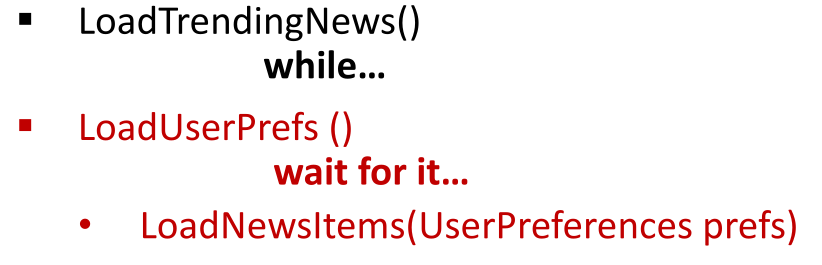
\includegraphics[width=0.5\textwidth]{async-news.png}
    \caption{}
\end{figure}


\subsubsection{Problem}

\begin{figure}[H]
    \centering
    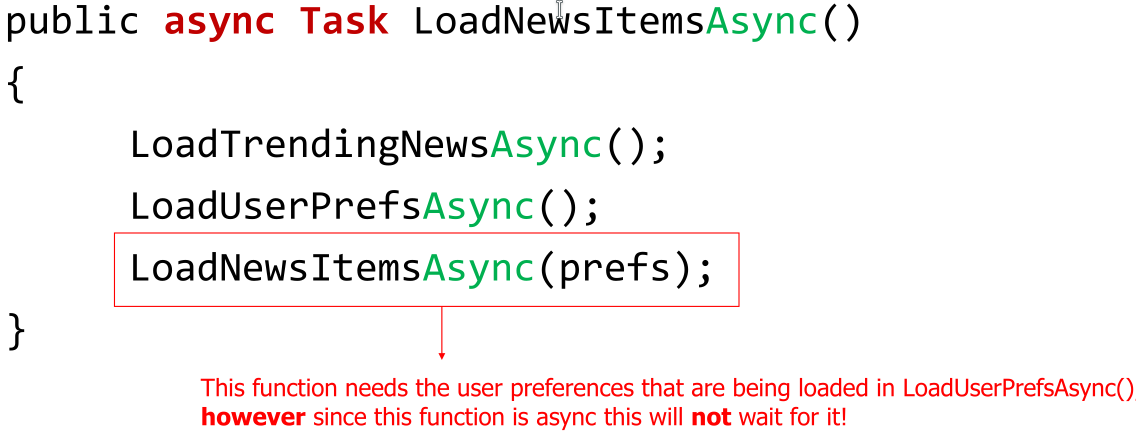
\includegraphics[width=0.7\textwidth]{async-news-problem.png}
    \caption{LoadNewsItemsAsync(prefs) needs to wait}
\end{figure}

\subsubsection{Solution}

\begin{figure}[H]
    \centering
    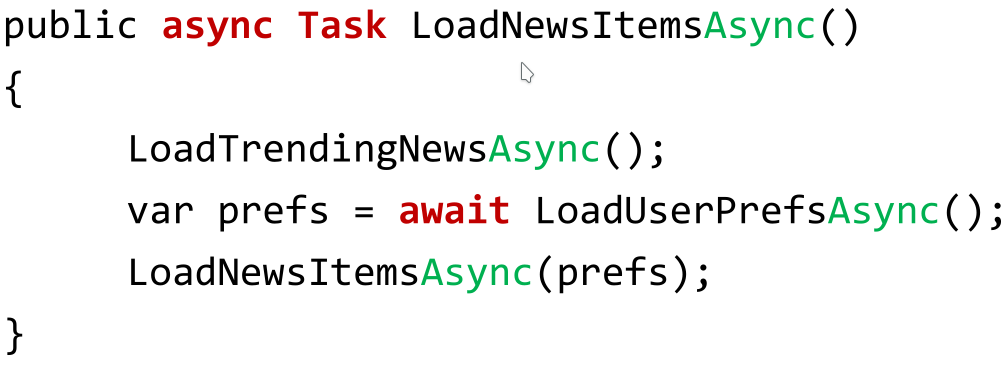
\includegraphics[width=0.7\textwidth]{async-news-solution.png}
    \caption{Solution: use the `await' keyword}
\end{figure}

\begin{figure}[H]
    \centering
    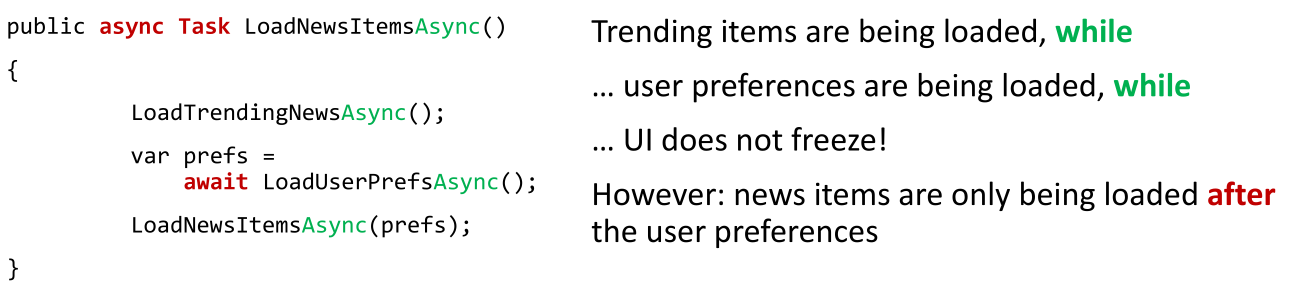
\includegraphics[width=0.8\textwidth]{async-news-solution2.png}
    \caption{}
\end{figure}

\subsection{Creating an asynchronous function}

\subsubsection{With void-functions: use Task}

\begin{figure}[H]
    \centering
    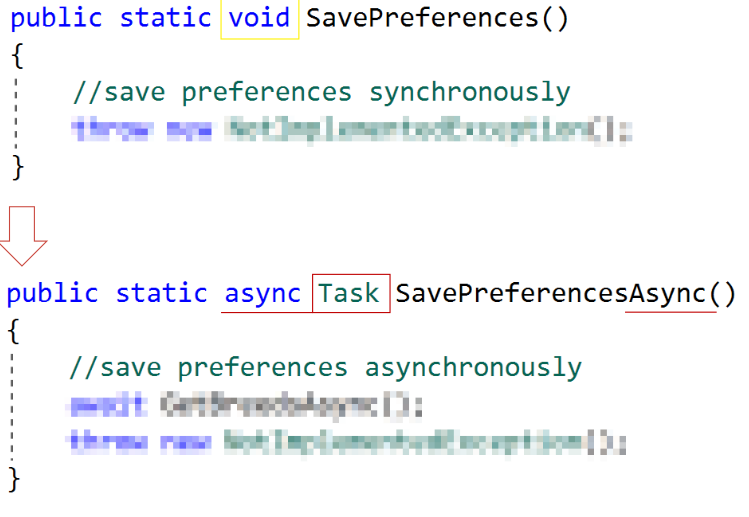
\includegraphics[width=0.6\textwidth]{async-void.png}
    \caption{Turning a void function asynchronous}
\end{figure}

\subsubsection{With a function that returns a type T}

\begin{figure}[H]
    \centering
    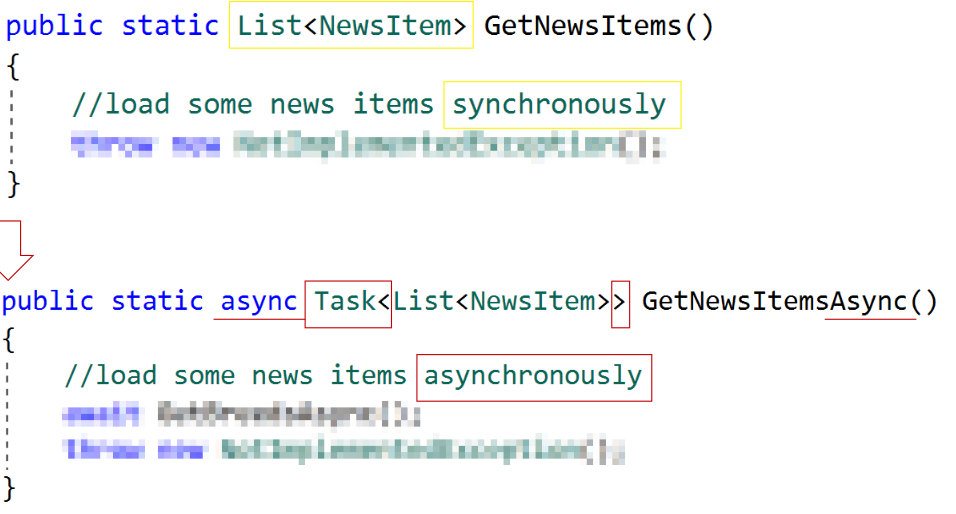
\includegraphics[width=0.7\textwidth]{async-type.png}
    \caption{Turning a type function asynchronous}
\end{figure}

\subsection{Calling an asynchronous function}

\begin{itemize}
    \item `async' in the headers of:
    \begin{itemize}
        \item the function you call it in (FillNewsItemsAsync)
        \item the function you are calling (GetNewsItemsAsync)
    \end{itemize}
    \item await when calling the function
\end{itemize}

\begin{figure}[H]
    \centering
    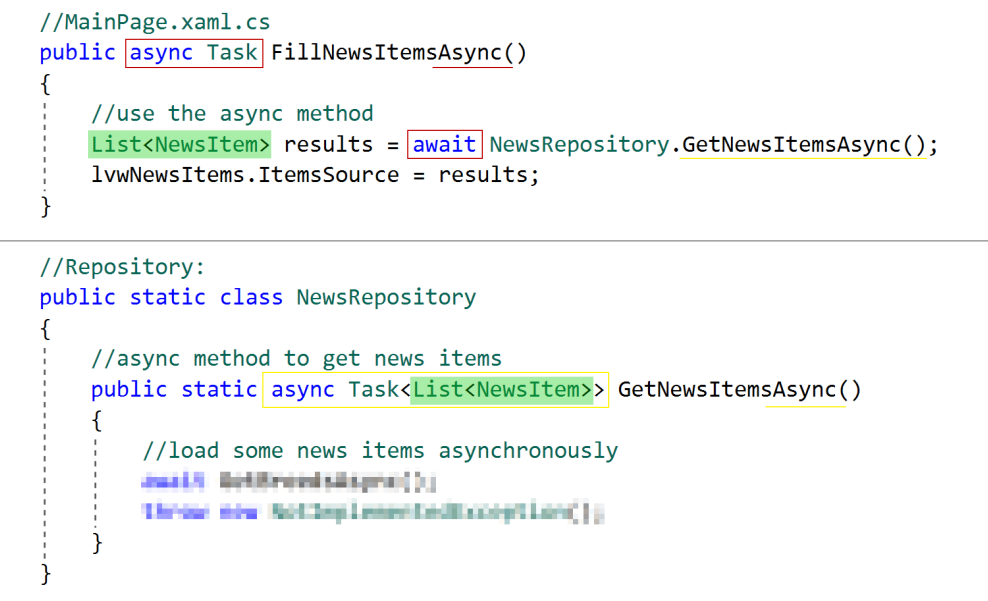
\includegraphics[width=0.5\textwidth]{async-calling.png}
    \caption{The await keyword}
\end{figure}

\subsection{Summary}
\begin{itemize}
    \item The difference between \bold{synchronous} and \bold{asynchronous} programming
    \item The \bold{what} and the \bold{why} of asynchronous programming
    \item The meaning and usage of the \bold{async} keyword
    \item The meaning and usage of the \bold{await} keyword
    \item The \bold{return type} of async functions
\end{itemize}

\section{XAML in Xamarin.Forms}

\begin{itemize}
    \item XAML was created by Microsoft specifically to describe UI
    \item Xamarin Forms + XAML = complete mobile app
\end{itemize}

\subsection{Benefits}

\begin{itemize}
    \item Seperation of UI from behaviour
    \item Easy designing of a UI, designer friendly
\end{itemize}

\subsection{Pages}

Xamarin.Forms Pages represent \bold{cross-platform} mobile application screens

\begin{figure}[H]
    \centering
    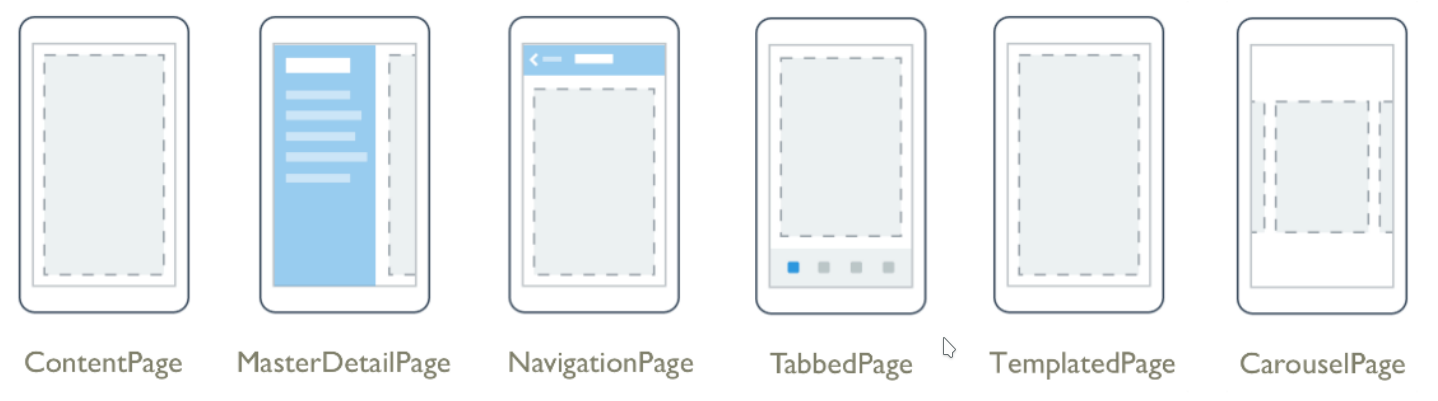
\includegraphics[width=0.5\textwidth]{xaml-page.png}
    \caption{Types of pages in Xamarin.Forms}
\end{figure}

\subsubsection{Adding a XAML Page}

There are two Item Templates available to add XAML Content

\begin{figure}[H]
    \centering
    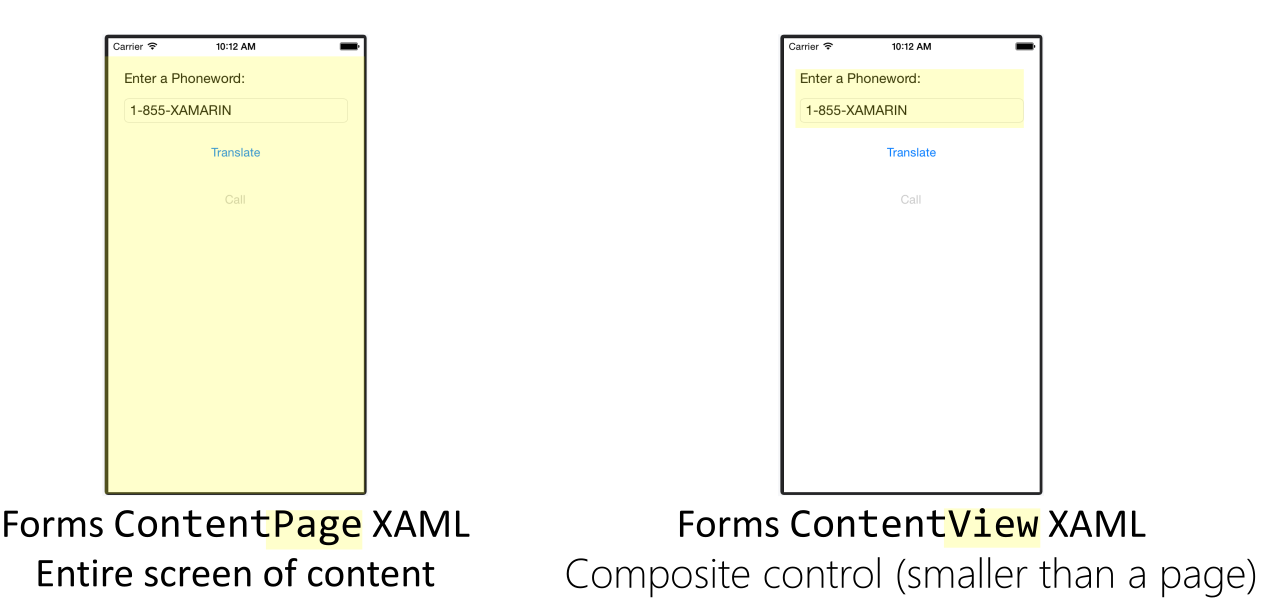
\includegraphics[width=0.4\textwidth]{contentpage-view.png}
    \caption{ContentPage vs ContentView}
\end{figure}

\subsection{Steps to build a UI with XAML}

\subsubsection{Describing a screen}

\begin{itemize}
    \item XAML is used to construct object graphs, in this case a visual Page
    \item XML based: case sensitive, open tags must be closed, etc \dots
\end{itemize}

\begin{figure}[H]
    \centering
    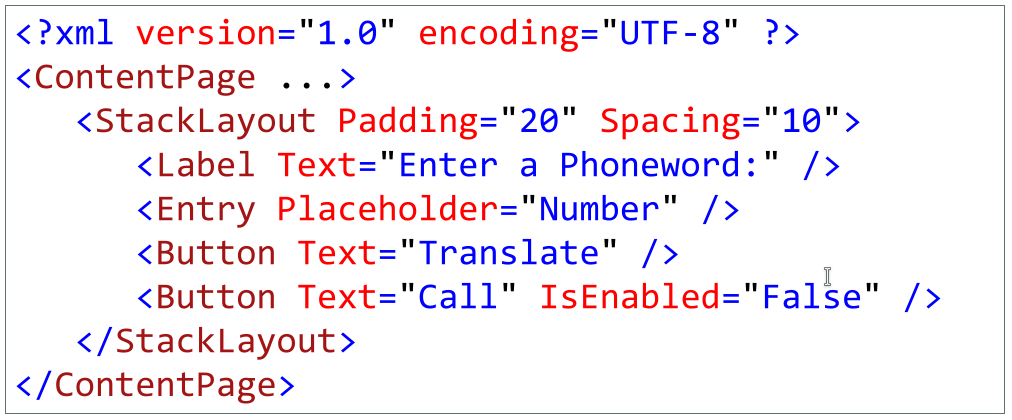
\includegraphics[width=0.4\textwidth]{xaml01.png}
    \caption{Example}
\end{figure}

\begin{figure}[H]
    \centering
    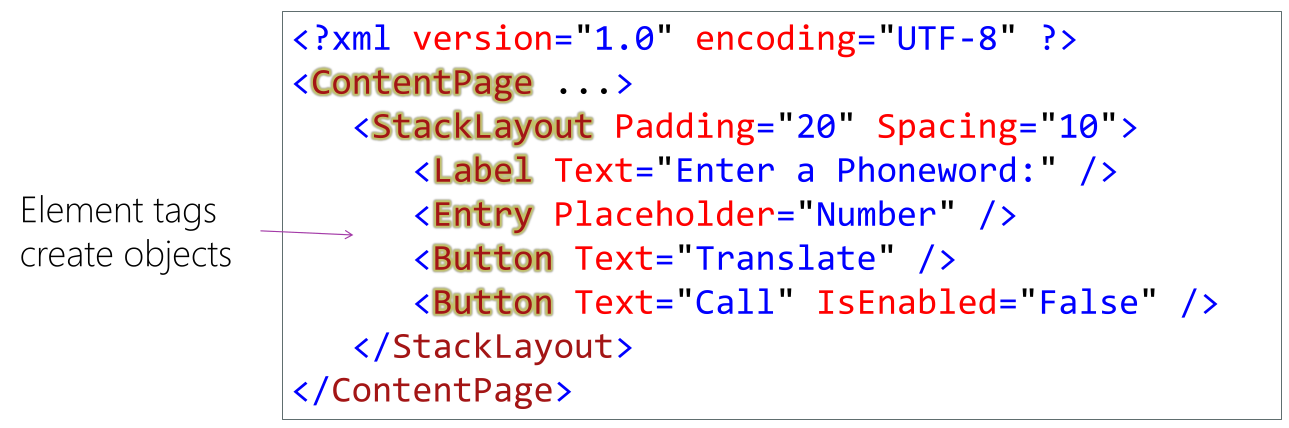
\includegraphics[width=0.5\textwidth]{xaml02.png}
    \caption{Element tags}
\end{figure}

\begin{figure}[H]
    \centering
    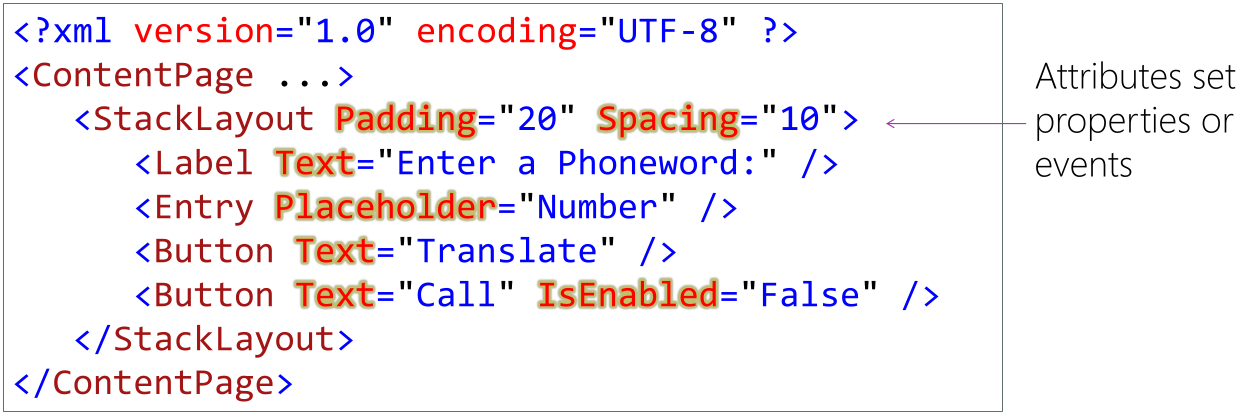
\includegraphics[width=0.5\textwidth]{xaml03.png}
    \caption{Attributes}
\end{figure}

\begin{figure}[H]
    \centering
    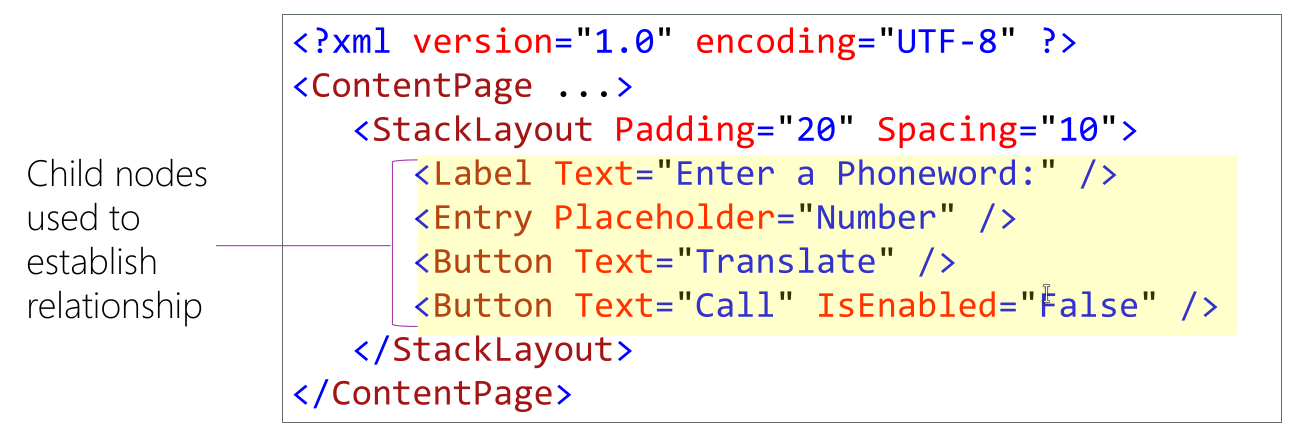
\includegraphics[width=0.5\textwidth]{xaml04.png}
    \caption{Child nodes in a StackLayout}
\end{figure}

\subsubsection{C\# code with XAML}

\begin{figure}[H]
    \centering
    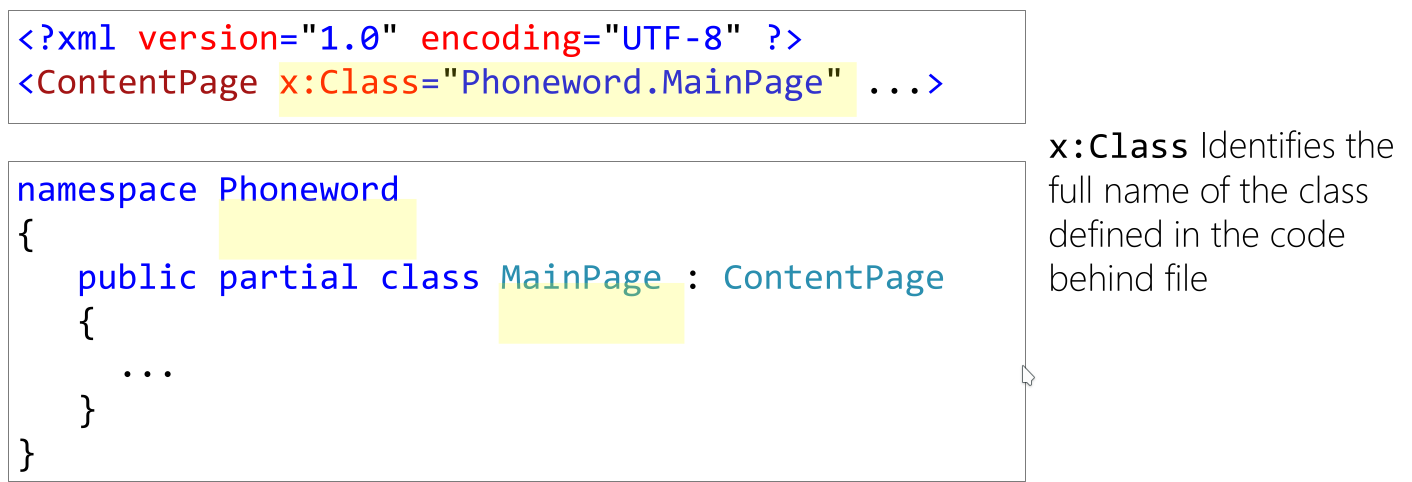
\includegraphics[width=0.5\textwidth]{xaml05.png}
    \caption{x:Class}
\end{figure}

\subsubsection{XAML Initialization}

The code behind the constructor has a call to `InitializeComponent' 
which is responsible for loading the XAML and creating the objects.
This method needs to run before doing anything else.

\begin{figure}[H]
    \centering
    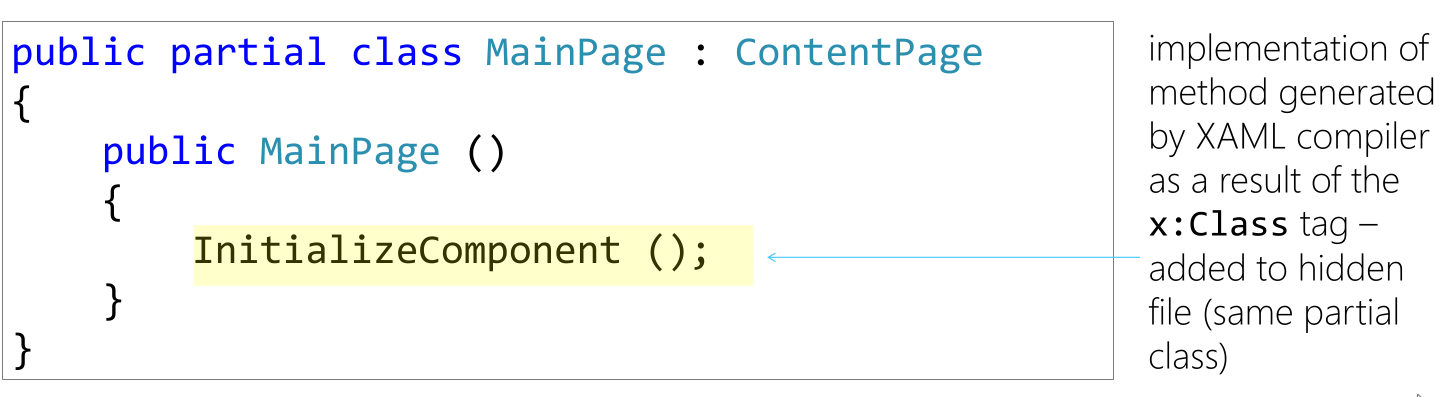
\includegraphics[width=0.5\textwidth]{xaml06.png}
    \caption{InitializeComponent}
\end{figure}

\subsubsection{Naming elements in XAML}

\begin{itemize}
    \item Use \bold{x:Name} to assign field name $\Rightarrow$ allows you to reference element in XAML and C\#
    \item This adds a private field to the XAML-generated partial class (file ending in \bold{.g.cs})
    \item Name must conform to C\# naming conventions
    \item Name must be unique
\end{itemize}

\begin{figure}[H]
    \centering
    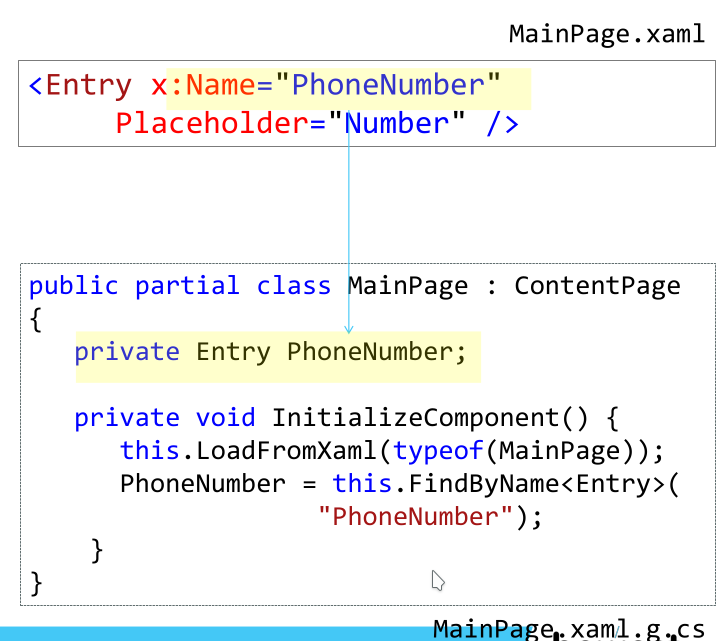
\includegraphics[width=0.4\textwidth]{xaml07.png}
    \caption{Naming elements}
\end{figure}

\subsubsection{Handling events in XAML}

\begin{itemize}
    \item You can wire up events in XAML
    \item The event handler must be defined in the C\# file and have proper signature
\end{itemize}

\begin{figure}[H]
    \centering
    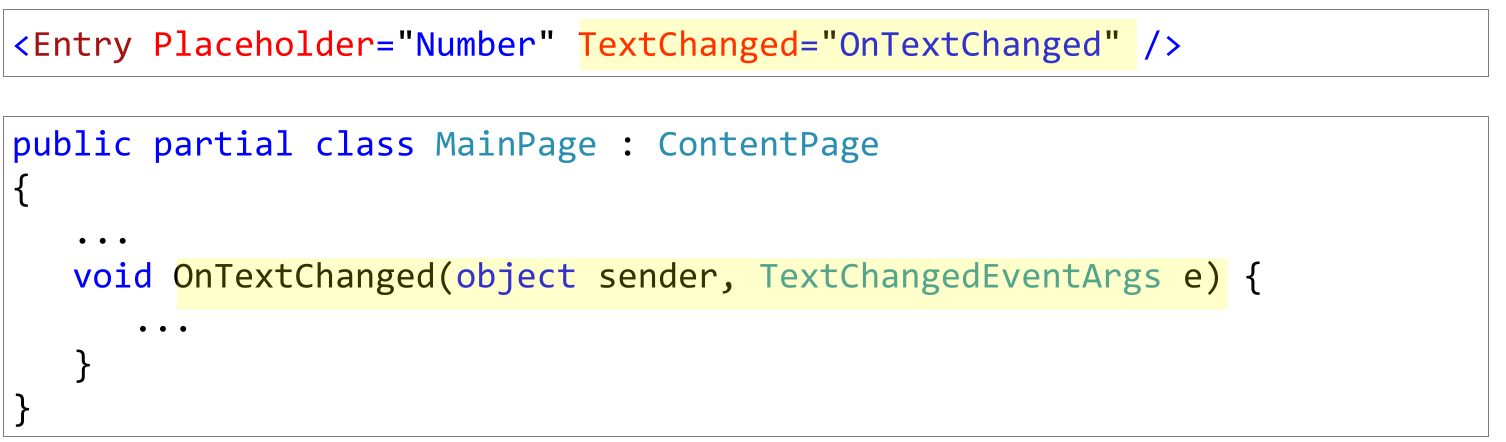
\includegraphics[width=0.5\textwidth]{xaml08.png}
    \caption{Event handling with the TextChanged Attribute}
\end{figure}

\subsubsection{Handling events in the code behind}

Can work with named elements as long as you define them in code, but keep in mind the field is not set until \bold{After} `InitializeComponent' is called

\begin{figure}[H]
    \centering
    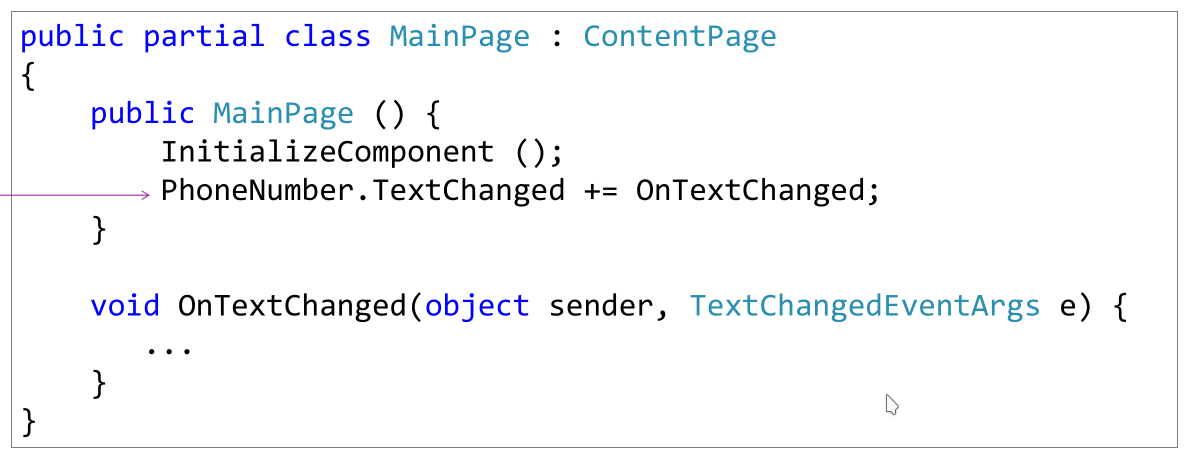
\includegraphics[width=0.5\textwidth]{xaml09.png}
    \caption{Adding event handler directly in code instead of in the XAML file}
\end{figure}

\begin{itemize}
    \item Many developers prefer to wire up all events in code behind by naming the XAML elements and adding event handlers in code
    \begin{itemize}
        \item Keeps the UI layer `pure' by pushing all behavior + management into the code behind
        \item Names are validated at compile time, but event handlers are not
        \item Easier to see how logic is wired up
    \end{itemize}
    \item Pick the approach that works for your team / preferences
\end{itemize}

\subsection{Layout in Xamarin.Forms}

\subsubsection{Motivation}
\begin{itemize}
    \item using layout containers to calculate view size and position helps your UI adapt to varied screen dimensions and resolutions
    \item Sizes/positions are recalculated automatically when device rotates
\end{itemize}

\subsubsection{Layouts}

A layout is a Xamarin.Forms container that determines the size and position for a collection of children

\begin{figure}[H]
    \centering
    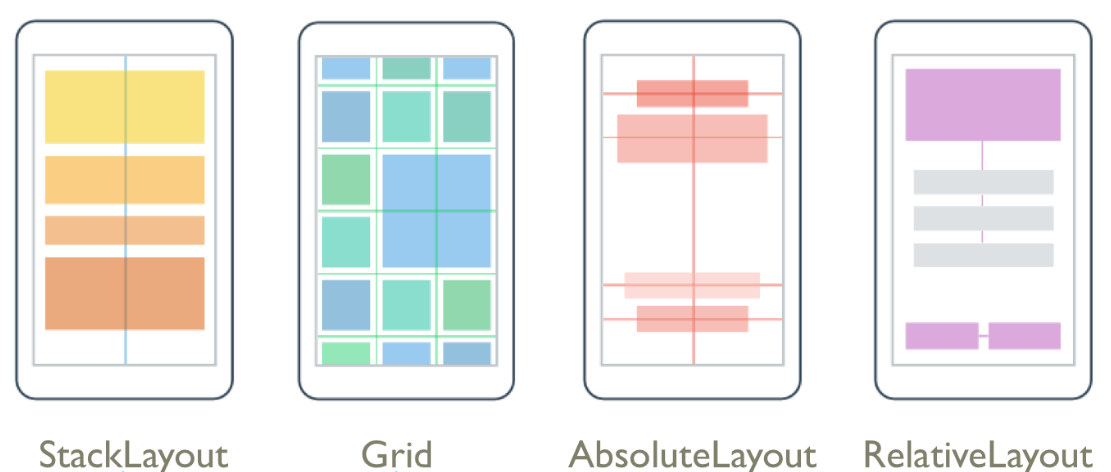
\includegraphics[width=0.5\textwidth]{xaml-layout.png}
    \caption{Layouts}
\end{figure}

\subsubsection{Views}

Views are the building blocks of cross-platform mobile user interfaces

\begin{itemize}
    \item User-interface objects such as labels, buttons, sliders, \dots
    \item Commonly known as controls or widgets in other graphical programming environments
\end{itemize}

\subsubsection{Working with sizes}

The rendered size of a view is a collaboration between the view itself and its layout container

\begin{figure}[H]
    \centering
    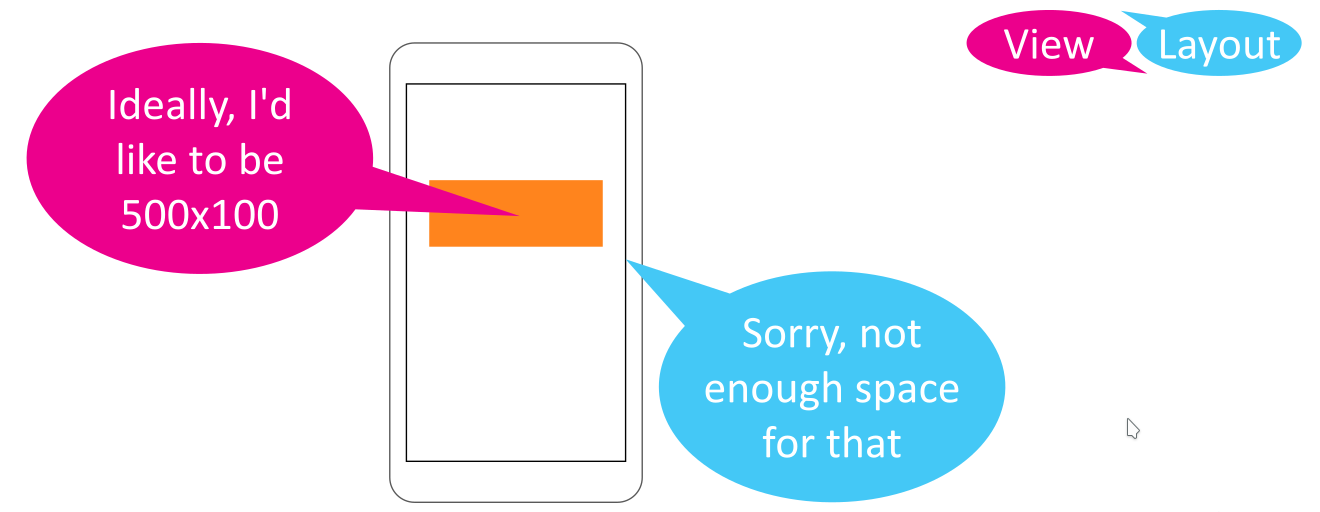
\includegraphics[width=0.5\textwidth]{xaml-view-sizing.png}
    \caption{XAML view vs sizing}
\end{figure}

\subsubsection{Layout algorithm}

\begin{enumerate}
    \item Layout panel asks each child how much room it would like
    \item Then tells each child how much it gets
\end{enumerate}


\begin{figure}[H]
    \centering
    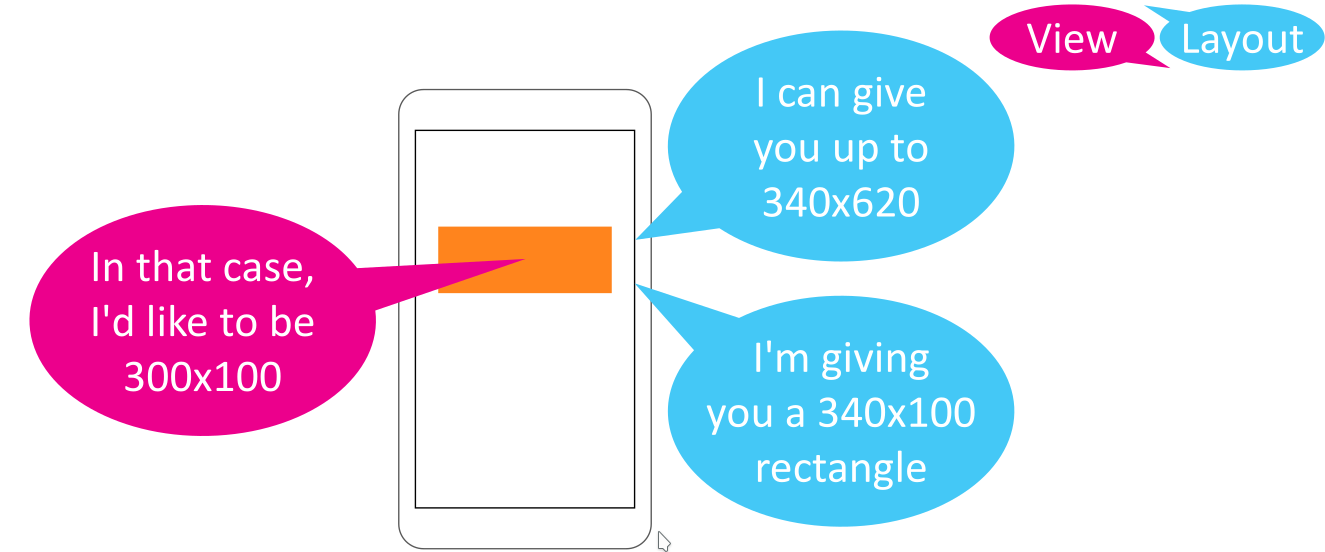
\includegraphics[width=0.5\textwidth]{xaml-view-layout.png}
    \caption{}
\end{figure}

\subsubsection{Default view sizing}

By default, most views try to size themselves just large enough to hold their content

\begin{figure}[H]
    \centering
    \includegraphics[width=0.5\textwidth]{xaml-default.png}
    \caption{Default sizing}
\end{figure}

\subsubsection{View preferences}

\begin{itemize}
    \item A view has four properties that influence its rendered size
    \item they are all requests and may be overruled by the layout container
\end{itemize}

\begin{figure}[H]
    \centering
    \includegraphics[width=0.5\textwidth]{xaml-view-preferences.png}
    \caption{View preferences using WidthRequest and HeightRequest, VerticalOptions and HorizontalOptions}
\end{figure}

\subsubsection{Sizing requests}

A view can request a desired with and height

\begin{figure}[H]
    \centering
    \includegraphics[width=0.5\textwidth]{xaml-sizing-requests.png}
    \caption{Preferred size}
\end{figure}

\subsubsection{Size units}

\begin{itemize}
    \item Explicit sizes in Xamarin.Forms have no intrinsic units
    \item The values are interpreted by each platform according to that platform's rules
    \begin{itemize}
        \item UWP: `Effective pixels'
        \item iOS: `Points'
        \item Android: `Density-independant pixels'
    \end{itemize}
\end{itemize}

\subsubsection{Platform rendering}
\begin{itemize}
    \item Sizes set in Xamarin.Forms are passed to the underlying platform
    \item The platform will scale the values based on screen size and resolution
\end{itemize}


\begin{figure}[H]
    \centering
    \includegraphics[width=0.5\textwidth]{xaml-platform-rendering.png}
    \caption{Platform rendering}
\end{figure}

\subsubsection{Alignment}

A view's preferred alignment determines its position and size within the rectangle allocated for it by its container

\begin{figure}[H]
    \centering
    \includegraphics[width=0.5\textwidth]{xaml-alingment.png}
    \caption{Alignment using HorizontalOptions}
\end{figure}


\subsubsection{Fill}


\begin{itemize}
    \item The `Fill' layout option generally overrides size preferences
    \item Horizontal and vertical alignment options generally default to Fill
\end{itemize}

\begin{figure}[H]
    \centering
    \includegraphics[width=0.5\textwidth]{xaml-fill.png}
    \caption{Fill overrides WidthRequest}
\end{figure}

\subsection{Margin \& Padding}

\subsubsection{Margin}

\begin{itemize}
    \item = extra space around the outside of a view
    \item available in all views, including containers
\end{itemize}

\begin{figure}[H]
    \centering
    \includegraphics[width=0.5\textwidth]{xaml-margins.png}
    \caption{Margins}
\end{figure}

\subsubsection{Padding}

\begin{itemize}
    \item = extra space on the inside of a layout that creates a gap between the children and the layout itself
    \item applicable only to layouts
\end{itemize}

\begin{figure}[H]
    \centering
    \includegraphics[width=0.5\textwidth]{xaml-padding.png}
    \caption{}
\end{figure}

\subsection{Arrange views with StackLayout}

StackLayout arranges its children in a single column or a single row

\begin{figure}[H]
    \centering
    \includegraphics[width=0.1\textwidth]{xaml-stacklayout.png}
    \caption{StackLayout}
\end{figure}


\subsubsection{Adding children}

\begin{figure}[H]
    \centering
    \includegraphics[width=0.5\textwidth]{xaml-stacklayout-children.png}
    \caption{Children in XAML}
\end{figure}

\subsubsection{Child ordering}

\begin{itemize}
    \item Child layout order is determined by the order they were added to the Children collection
    \item Applies to both code and XAML
\end{itemize}

\subsubsection{Child spacing}

\begin{itemize}
    \item StackLayout's Spacing separates the children
    \item The default is 6
\end{itemize}

\begin{figure}[H]
    \centering
    \includegraphics[width=0.5\textwidth]{xaml-stacklayout-spacing.png}
    \caption{Add space between children}
\end{figure}

\subsubsection{Orientation}



\begin{itemize}
    \item StackLayout's Orientation property lets you choose a vertical column or a horizontal row
    \item Vertical is the default
\end{itemize}

\begin{figure}[H]
    \centering
    \includegraphics[width=0.5\textwidth]{xaml-stacklayout-orientation.png}
    \caption{}
\end{figure}

\bold{LayoutOptions with and against orientation}

\begin{itemize}
    \item In the direction opposite of its orientation, StackLayout uses the \bold{Start}, \bold{Center}, \bold{End} and \bold{Fill} layout options
    \item In the direction of its orientation, StackLayout ignores the Start, Center, End, and Fill layout options
\end{itemize}

\begin{figure}[H]
    \centering
    \includegraphics[width=0.5\textwidth]{xaml-stacklayout-orientation3.png}
    \caption{With orientation}
\end{figure}

\begin{figure}[H]
    \centering
    \includegraphics[width=0.5\textwidth]{xaml-stacklayout-orientation2.png}
    \caption{Against orientation}
\end{figure}


\subsection{Expansion}

\begin{itemize}
    \item A view's \bold{expansion setting} determines whether it would like the StackLayout to allocate available extra space to its rectangle
\end{itemize}

\begin{figure}[H]
    \centering
    \includegraphics[width=0.5\textwidth]{xaml-expansion.png}
    \caption{Expansion}
\end{figure}

\subsubsection{Expansion direction}

\begin{itemize}
    \item StackLayout expands children only in the direction of its orientation
    \item For example: a vertical StackLayout expands vertically
\end{itemize}

\subsubsection{How much extra space?}

StackLayout determines the amount of extra space using its standard layout calculation as if there were no expansion

\begin{figure}[H]
    \centering
    \includegraphics[width=0.5\textwidth]{xaml-expansion-space.png}
    \caption{Amount of extra space}
\end{figure}

\subsubsection{How to specify expansion?}

To request expansion, use the "...AndExpand" version of the layout options in the direction of the StackLayout's orientation

\begin{figure}[H]
    \centering
    \includegraphics[width=0.5\textwidth]{xaml-expansion-specify.png}
    \caption{}
\end{figure}

\subsubsection{Expansion vs view size}

\begin{itemize}
    \item Enabling expansion can change the size of the view's layout rectangle, but doesn't change the size of the view unless it uses FillAndExpand
    \item In the direction \bold{opposite} its orientation, adding "...AndExpand" tot the layout options has no effect (there is no expansion in that direction)
\end{itemize}

\begin{figure}[H]
    \centering
    \includegraphics[width=0.5\textwidth]{xaml-expansion-viewsize.png}
    \caption{}
\end{figure}

\subsection{Apply attached properties}

\subsubsection{Motivation}

Some properties are only needed in specific situations

\begin{figure}[H]
    \centering
    \includegraphics[width=0.5\textwidth]{xaml-attachedproperties.png}
    \caption{}
\end{figure}

\subsubsection{What is an attached property?}

= a property that is defined in one class but set on objects of other types

\begin{itemize}
    \item Button does not have Row/Column properties
    \item They are defined in Grid and attached to objects of other types as needed
    \begin{itemize}
        \item Grid.Row="0", Grid.Row="1", \dots
    \end{itemize}
\end{itemize}

\subsubsection{Who consumes attached properties?}

Typically, a container will look for attached properties on its children

\begin{figure}[H]
    \centering
    \includegraphics[width=0.5\textwidth]{xaml-attachedproperties2.png}
    \caption{}
\end{figure}

\subsubsection{Apply an attached property in code}

In code, use the static Set method to apply an attached property

\begin{figure}[H]
    \centering
    \includegraphics[width=0.5\textwidth]{xaml-attachedproperties3.png}
    \caption{Attached property in code}
\end{figure}

\subsubsection{Apply an attached property in XAML}

In XAML, use the owning class name and the attached property name (without the Property suffix)

\begin{figure}[H]
    \centering
    \includegraphics[width=0.5\textwidth]{xaml-attachedproperties3.png}
    \caption{Attached property in XAML}
\end{figure}

\subsection{Grids}

Grid places its children into cells formed from rows and columns

\begin{figure}[H]
    \centering
    \includegraphics[width=0.1\textwidth]{xaml-grid1.png}
    \caption{}
\end{figure}

\subsubsection{Grid rows/columns}

You specify the shape of the grid by defining each row and column individually

\begin{figure}[H]
    \centering
    \includegraphics[width=0.4\textwidth]{xaml-grid2.png}
    \caption{}
\end{figure}

There are dedicated classes that define a row or a column

\begin{figure}[H]
    \centering
    \includegraphics[width=0.5\textwidth]{xaml-grid-rowcol.png}
    \caption{RowDefinition and ColumnDefinition}
\end{figure}

\subsubsection{GridLength}

GridLength encapsulates two things: unit and value

\begin{figure}[H]
    \centering
    \includegraphics[width=0.5\textwidth]{xaml-grid-length.png}
    \caption{}
\end{figure}

\bold{Absolute GridLength}

Absolute GridLength specifies a fixed row height or column width

\begin{figure}[H]
    \centering
    \includegraphics[width=0.5\textwidth]{xaml-grid-length-abs.png}
    \caption{Absolute GridLength}
\end{figure}

\bold{Auto GridLength}

Auto GridLength lets the row height or column width adapt, it automatically
becomes the size of the largest child

\begin{figure}[H]
    \centering
    \includegraphics[width=0.5\textwidth]{xaml-grid-length-auto.png}
    \caption{Auto GridLength}
\end{figure}

\bold{Star (*) GridLength}

Star GridLength shares the available space proportionally among all rows/columns
that use star sizing

\begin{figure}[H]
    \centering
    \includegraphics[width=0.5\textwidth]{xaml-grid-length-star.png}
    \caption{Star GridLength}
\end{figure}

\subsubsection{Grid example}

It is common to mix different GridLength settings in the same grid

\begin{figure}[H]
    \centering
    \includegraphics[width=0.5\textwidth]{xaml-grid-example.png}
    \caption{}
\end{figure}

\subsubsection{Default size}

Rows and columns default to \bold{`1*'} size

\begin{figure}[H]
    \centering
    \includegraphics[width=0.5\textwidth]{xaml-grid-defaultsize.png}
    \caption{}
\end{figure}

\subsubsection{Row/Column numbering}

Starts at 0:

\begin{figure}[H]
    \centering
    \includegraphics[width=0.2\textwidth]{xaml-grid-numbering.png}
    \caption{}
\end{figure}

\subsubsection{Grid positioning properties}

Grid defines four attached properties used to position children

\begin{figure}[H]
    \centering
    \includegraphics[width=0.5\textwidth]{xaml-grid-pos-props.png}
    \caption{}
\end{figure}

\subsubsection{Cell specification}

Apply the Row and Column attached properties to each child

\begin{figure}[H]
    \centering
    \includegraphics[width=0.5\textwidth]{xaml-grid-cells.png}
    \caption{}
\end{figure}

\subsubsection{Span specification}

Apply RowSpan and ColumnSpan to each child as needed

\begin{figure}[H]
    \centering
    \includegraphics[width=0.5\textwidth]{xaml-grid-span.png}
    \caption{}
\end{figure}

\subsubsection{Cell and span defaults}

Cell locations default to 0 and spans default to 1

\begin{figure}[H]
    \centering
    \includegraphics[width=0.5\textwidth]{xaml-grid-cell-span-defaults.png}
    \caption{}
\end{figure}

\subsubsection{Layout options}

A view's horizontal and vertical layout options control how it is sized and positioned within its grid cell (the default is Fill)

\begin{figure}[H]
    \centering
    \includegraphics[width=0.5\textwidth]{xaml-grid-layout.png}
    \caption{}
\end{figure}

\subsubsection{Grid child spacing}

\begin{itemize}
    \item Grid's RowSpacing and ColumnSpacing properties separate the children
    \item They both default to 6
\end{itemize}

\begin{figure}[H]
    \centering
    \includegraphics[width=0.5\textwidth]{xaml-grid-child-spacing.png}
    \caption{}
\end{figure}

\subsubsection{Auto-generated rows/columns}

Grid will automatically generate equal-sized rows/columns based on the position of the children you add

\begin{figure}[H]
    \centering
    \includegraphics[width=0.5\textwidth]{xaml-grid-autogenerated.png}
    \caption{}
\end{figure}

\subsection{Scroll a layout with ScrollView}

ScrollView adds scrolling to a single piece of content; the content can be an
individual view or a layout container

\subsubsection{How to use ScrollView}

Wrap a ScrollView around a single element to add scrolling

\begin{figure}[H]
    \centering
    \includegraphics[width=0.5\textwidth]{xaml-scrollview.png}
    \caption{}
\end{figure}

\subsubsection{ScrollView orientation}

ScrollView lets you control the scroll direction: 

\begin{itemize}
    \item Vertical (the default)
    \item Horizontal
    \item or Both
\end{itemize}


\begin{figure}[H]
    \centering
    \includegraphics[width=0.5\textwidth]{xaml-scrollview-orientation.png}
    \caption{}
\end{figure}


\subsubsection{Do not nest scrolling views}

Generally, do not nest ScrollViews or a ListView in a ScrollView, it often
creates non-intuitive behavior

\begin{figure}[H]
    \centering
    \includegraphics[width=0.5\textwidth]{xaml-scrollview-nest.png}
    \caption{This is bad practice}
\end{figure}


\subsection{Summary}

\begin{itemize}
    \item Examining XAML syntax
    \item Adding Behavior to XAML-based pages
    \item Exploring XAML capabilities
    \item Specify the size of a view
    \item Arrange views with StackLayout
    \item Apply Attached Properties
    \item Arrange views with Grid
    \item Scroll a layout with ScrollView
\end{itemize}

\end{document}